%%=============================================================================
%% Excitation-Aware On-Track System Identification at Full Scale
%%
%% International Journal of Dynamics and Control, Springer Nature sn-jnl class.
%% One .tex document, figures attached separately under Figures/, and blinded
%% for the journal's double-blind review: the author block, the affiliations
%% and the acknowledgements are in sn-title-page.tex instead.
%%
%% Build: pdflatex main && bibtex main && pdflatex main && pdflatex main
%%=============================================================================
\documentclass[lineno,12pt]{sn-jnl}

\usepackage{cite}%
\usepackage{graphicx}%
\usepackage{multirow}%
\usepackage{amsmath,amssymb,amsfonts}%
\usepackage{amsthm}%
\usepackage{mathrsfs}%
\usepackage[title]{appendix}%
\usepackage{xcolor}%
\usepackage{textcomp}%
\usepackage{manyfoot}%
\usepackage{booktabs}%
\usepackage{array}%

% --- notes under a table ------------------------------------------------------
% sn-jnl loads threeparttable and then redefines \tabular, which leaves the
% package's saved \tabular defined in terms of itself: the second
% threeparttable of the document recurses until TeX runs out of grouping
% levels. Both environments are therefore replaced by the plain block of note
% paragraphs the Springer template asks for, which keeps every table body in
% this manuscript unchanged.
\makeatletter
\renewenvironment{threeparttable}{}{}
\renewenvironment{tablenotes}[1][]{%
  \par\vspace{2pt}\begingroup
  % The enclosing table sets \centering, whose \leftskip and \rightskip
  % survive a plain \raggedright here, so the glue is set directly.
  \leftskip\z@ \@rightskip\@flushglue \rightskip\@rightskip
  \parfillskip\@flushglue \parindent\z@
  \def\item{\par\noindent}\ignorespaces}%
  {\par\endgroup}
\makeatother

% --- lightweight algorithm float ---------------------------------------------
% float.sty ships with texlive-latex-recommended; the algorithm/algorithmicx
% families do not, so the body of Algorithm 1 is plain LaTeX rather than a new
% dependency.
\usepackage{float}%
\newfloat{algorithm}{tbp}{loa}
\floatname{algorithm}{Algorithm}
\newcommand{\algline}[2]{\makebox[1.8em][r]{\scriptsize#1:}\ \ #2\par}
\newcommand{\algin}[1]{\hspace*{#1em}}

% --- units -------------------------------------------------------------------
% Minimal siunitx replacement, implementing exactly the macros this manuscript
% uses. siunitx ships in texlive-science rather than texlive-latex-extra, so it
% cannot be assumed present; where it is, replacing this block with
% \usepackage{siunitx} plus \sisetup{detect-all, per-mode=symbol} and
% \DeclareSIUnit{\g}{\textit{g}} typesets the same units.
% All macros are robust: a table caption is a moving argument, and an
% expandable conditional breaks there.
\makeatletter
% Armed once a base unit has been emitted, disarmed after a prefix and after
% \per, so "kilo newton per radian" sets no space between k and N nor around
% the solidus.
\newif\ifsiu@prev
\DeclareRobustCommand{\siu@sep}{\ifsiu@prev\,\fi}
% \text{} so a unit typesets upright in both text and math mode: these macros
% are routinely used inside $...$, where a bare `m' would come out as an italic
% math variable.
\DeclareRobustCommand{\siu@unit}[1]{\siu@sep\text{#1}\siu@prevtrue}
\DeclareRobustCommand{\siu@pre}[1]{\siu@sep\text{#1}\siu@prevfalse}
\DeclareRobustCommand{\siu@div}[1]{\text{#1}\siu@prevfalse}
\DeclareRobustCommand{\meter}{m}
\DeclareRobustCommand{\second}{s}
\DeclareRobustCommand{\gram}{g}
\DeclareRobustCommand{\newton}{N}
\DeclareRobustCommand{\radian}{rad}
\DeclareRobustCommand{\hertz}{Hz}
\DeclareRobustCommand{\percent}{\%}
\DeclareRobustCommand{\g}{\textit{g}}
\DeclareRobustCommand{\kilo}{k}
\DeclareRobustCommand{\milli}{m}
\DeclareRobustCommand{\per}{/}
\DeclareRobustCommand{\squared}{\ensuremath{^{2}}}
\providecommand{\degree}{\ensuremath{^{\circ}}}
\DeclareRobustCommand{\si}[1]{\begingroup
  \siu@prevfalse
  \renewcommand{\meter}{\siu@unit{m}}%
  \renewcommand{\second}{\siu@unit{s}}%
  \renewcommand{\gram}{\siu@unit{g}}%
  \renewcommand{\newton}{\siu@unit{N}}%
  \renewcommand{\radian}{\siu@unit{rad}}%
  \renewcommand{\hertz}{\siu@unit{Hz}}%
  \renewcommand{\percent}{\siu@unit{\%}}%
  \renewcommand{\degree}{\siu@unit{\ensuremath{^{\circ}}}}%
  \renewcommand{\g}{\siu@unit{\textit{g}}}%
  \renewcommand{\kilo}{\siu@pre{k}}%
  \renewcommand{\milli}{\siu@pre{m}}%
  \renewcommand{\per}{\siu@div{/}}%
  \renewcommand{\squared}{\ensuremath{^{2}}}%
  #1\endgroup}
\DeclareRobustCommand{\num}[1]{#1}
\DeclareRobustCommand{\numrange}[2]{#1\text{--}#2}
\DeclareRobustCommand{\SI}[2]{#1\,\si{#2}}
\DeclareRobustCommand{\SIrange}[3]{#1\text{--}#2\,\si{#3}}
\makeatother

\hyphenation{op-tical net-works semi-conduc-tor Pa-cej-ka iden-ti-fi-ca-tion}

% --- convenience macros -------------------------------------------------------
\newcommand{\vecx}{\mathbf{x}}
\newcommand{\vecu}{\mathbf{u}}
\newcommand{\vecz}{\mathbf{z}}
\newcommand{\phip}{\Phi_{p}}
\newcommand{\Fyf}{F_{y,f}}
\newcommand{\Fyr}{F_{y,r}}
% Blinded names. The simulator bridge and the identification package are named
% in sn-title-page.tex and in the unblinded release; here they carry names that
% do not identify the institution or the repository owner.
\newcommand{\bridge}{\textsc{SimBridge}}
\newcommand{\sysid}{\textsc{On-Track-SysID}}
% --- benchmark arm names -------------------------------------------------------
\newcommand{\oursarm}{\texttt{Excitation-\allowbreak S4D-\allowbreak Pinn}}
\newcommand{\basearm}{\texttt{Baseline-\allowbreak NN-\allowbreak MSE}}

\theoremstyle{thmstyleone}%
\newtheorem{theorem}{Theorem}%
\newtheorem{proposition}[theorem]{Proposition}%
\theoremstyle{thmstyletwo}%
\newtheorem{example}{Example}%
\newtheorem{remark}{Remark}%
\theoremstyle{thmstylethree}%
\newtheorem{definition}{Definition}%

% The floats here are large and every one of them is read against the
% paragraph it sits in, so the default fractions, which reserve a fifth of each
% page for text and defer anything larger, would push most of them past the end
% of the section that discusses them.
\renewcommand{\topfraction}{0.9}
\renewcommand{\bottomfraction}{0.8}
\renewcommand{\textfraction}{0.07}
\renewcommand{\floatpagefraction}{0.75}
\setcounter{topnumber}{3}
\setcounter{bottomnumber}{2}
\setcounter{totalnumber}{5}

\raggedbottom

\begin{document}

\title[Excitation-Aware On-Track System Identification at Full Scale]{Excitation-Aware On-Track System Identification at Full Scale: A Simulation Study}

%%=============================================================%%
%% Double-blind review: the author block, the affiliations, the
%% acknowledgements and the funding statement are in sn-title-page.tex.
%%=============================================================%%

\abstract{On-track system identification learns tire models from ordinary
racing laps instead of dedicated manoeuvres. We study one such
residual-learning pipeline at full vehicle scale, inside a simulator that
publishes per-wheel forces as ground truth. Transplanted unchanged from a 1:10
platform, it converges on a tire with less than half the vehicle's grip ceiling
and most Pacejka coefficients resting on their bounds. The cause is a loss of
excitation created by the pipeline's own virtual-data step: the friction the
synthetic rollout can demand is a property of the rollout configuration and not
of the tire, as a grid on a known tire confirms. Two further defects share that
source. The objective the coefficients are fitted against depends on them only
through one product, so the peak factor is not recoverable from the rollout at
any excitation, and the loop that feeds each fit its own previous answer is not
a contraction. We correct all three, and gate the controller interface on
derived physical quantities rather than on coefficient bounds. On a static
surface 33\% below the one the tire prior was measured on, axle cornering
stiffness is recovered to within 3.2\% and the peak factor to 11\%. On a
surface losing half its grip under the moving vehicle, the corrected pipeline
tracks the decay rate to 7\% and completes three timed laps at unchanged
lateral tracking error for 18\% of lap time, where the inherited configuration
holds a grip ceiling nearly four times the plant's and leaves the track.}

\keywords{System identification, Tire models, Vehicle dynamics, Autonomous
racing, Model predictive control, Persistent excitation}

\maketitle

% === I. INTRODUCTION =========================================================
\section{Introduction}

Model-based controllers for autonomous racing derive their
performance from the fidelity of the vehicle model they carry
\cite{liniger2015,kabzan2019lbmpc,forzaeth2024}. In the lateral channel that
fidelity is dominated by the tire, simultaneously the physical bound on
manoeuvrability and the least accessible component to measure
\cite{pacejka2012book,amz2020}. Classical characterisation takes the vehicle
off the track for steady-state circular or ramp-steer manoeuvres, at a
logistical cost a race weekend rarely affords; identifying on track removes the
logistics but brings back transients, noise and a racing line that is a poor
excitation signal, and nonlinear least squares applied directly to lap data is
brittle in exactly this regime \cite{ontrack2025}.

Dikici \emph{et al.}~\cite{ontrack2025} propose the hybrid remedy that is the
starting point of this paper: a small residual network trained on
\SI{30}{\second} of ordinary lap data predicts the one-step error of a nominal
single-track model; the corrected model is rolled out through a \emph{synthetic}
quasi-steady steering sweep; Pacejka coefficients are fitted to that sweep; and
each fit becomes the next nominal model. Because the sweep is generated rather
than driven it can be made steady and noise-free, and the residual network only
has to interpolate within its training distribution. On a 1:10 platform the
procedure reports a \num{3.3}$\times$ lower one-step RMSE than nonlinear least
squares under noise \cite{ontrack2025}.

\subsection{Problem statement}

This paper asks what the pipeline identifies when it is moved from a
\SI{3.7}{\kilo\gram}, \SI{0.32}{\meter}-wheelbase platform to a full-scale
Formula Student vehicle: \SI{269.6}{\kilo\gram}, \SI{1.53}{\meter} wheelbase,
\SI{16}{\degree} of road-wheel lock, following a reference speed profile of
\SIrange{9.6}{25.8}{\meter\per\second}. The question is identifiability, not
parameter transfer, and two scale-dependent mechanisms, both latent at 1:10,
break the estimate. First, excitation collapses inside the virtual-data
step: the Pacejka fit never sees the recorded lap, only the synthetic rollout,
whose reachable friction
$\mu_{\mathrm{reach}}\!\approx\!v^{2}\delta_{\mathrm{sweep}}/(gL)$ is a property
of the rollout configuration and not of the tire, and a rollout speed inherited
from the scaled platform caps it at $0.43$ here. Below the tire's peak the Magic
Formula degenerates to $F_{y}\approx F_{z}(BCD)\alpha$, only the product $BCD$
is identifiable, and the bounded optimiser resolves the remaining freedom on a
box edge \cite{ljung1999sysid,pacejka2012book}. Second, lateral demand
scales as $v^{2}$, so the tracking cost of a bad grip estimate grows
quadratically with speed:
one identified set with a peak friction coefficient of \num{0.40} tracked at
\SI{0.16}{\meter} of cross-track error at \SI{11.1}{\meter\per\second} and
\SI{41.89}{\meter} at \SI{27}{\meter\per\second} through the same controller
(Section~\ref{subsec:gates}), and the scaled platform never reaches the speed at
which that error becomes observable.

One difference works in our favour. Because the study runs in the CARLA
simulator \cite{carla2017} through a purpose-built ROS~2 interface, the
simulator's own per-wheel telemetry (slip angle, normal load and lateral force)
is available as ground truth, so an on-track identifier can be scored against
the forces the plant actually generated.

\subsection{Contributions}

\begin{enumerate}
\item \textbf{An identifiability analysis of the virtual-data step}
(Section~\ref{subsec:excitation}): the closed-form reachable-friction bound
above, and an \emph{excitation-aware rollout} that selects the rollout speed
from the measured lap and warns when the configuration cannot reach the prior's
peak. A grid over rollout speed, sweep amplitude and true peak factor on a known
tire both verifies the bound and selects the rollout speed floor and sweep-amplitude
ceiling the pipeline ships (Section~\ref{subsec:sweep}). This corrects the baseline
method~\cite{ontrack2025} at any scale, and stays latent at 1:10 because a
\SIrange{2}{4}{\meter\per\second} rollout is representative there and is not
here.

\item \textbf{Two structural properties of the loop, and the corrections they
imply} (Section~\ref{subsec:contraction}): stage~3's residual depends on $B$,
$C$ and $D$ only through their product, so the peak factor is not recoverable
from the rollout \emph{at any excitation} and must be measured on the recorded
trace and held; and the loop is a positive feedback path rather than a
contraction, so stage~4 becomes a relaxed fixed-point iteration at
$\beta=\num{0.20}$.

\item \textbf{The corrections the bound implies}, on both sides of the fit
(Sections~\ref{subsec:iterative} and~\ref{subsec:measurement}): a sweep bounded
at $1.5\times$ the 99th percentile of the observed steering, a Tikhonov target
frozen at the configured prior, slip angles built from the \emph{achieved}
road-wheel angle, mass and wheelbase from measured static wheel loads, a
friction warm start from the \emph{curvature} of the axle force curve, and
physics-informed dynamics residuals normalised to the state-increment units of
the data term, from which raw force and moment residuals sit a factor
$\num{2.3}\times10^{5}$ away.

\item \textbf{Admissibility gates on derived physical quantities} at the
model-to-controller boundary (Section~\ref{sec:integration}): axle cornering
stiffness, understeer sign and critical speed, and grip ceiling against the
trajectory's lateral demand. They replace per-coefficient box checks, which
cannot detect a degenerate fit or a pairwise-oversteering axle set.

\item \textbf{A simulation architecture that supplies the ground truth, and a
closed-loop evaluation on two surfaces}
(Sections~\ref{subsec:platform}--\ref{subsec:data} and~\ref{sec:results}). The
first is static at \num{0.70}, deliberately not the \num{1.05} the configured
tire prior was measured on, so a pipeline unable to move off its prior scores
badly. Over three timed laps the corrected pipeline identifies axle cornering
stiffness to \SI{3.2}{\percent} front and \SI{1.4}{\percent} rear and tracks
the peak factor to \SI{11}{\percent}, against an inherited configuration that
rails $D$ on its \num{2.0} bound in every cycle and overstates stiffness by
\SIrange{118}{132}{\percent}; axle force RMSE is \num{12.1}$\times$ and
\num{10.5}$\times$ lower and MPC lateral tracking error \SI{32}{\percent}
lower, at unchanged solver cost. On the second the bridge drives the plant's
friction down under a moving vehicle on the linear-decay protocol
of~\cite{llampc2025} until half the grip is gone. The corrected pipeline
recovers the decay \emph{rate} to \SI{7}{\percent}, which a single surface
cannot test at any accuracy, and the level to
\SIrange{10.9}{17.4}{\percent} once one identification cycle of transport lag is
accounted for. The falling peak factor then re-clamps the reference speed
profile from \SI{0.51}{\g} of peak lateral demand to \SI{0.30}{\g}, and the
vehicle finishes three laps at unchanged tracking error for \SI{18}{\percent}
of lap time. The inherited configuration cannot make that trade, because a peak
factor resting on a box constraint reports no change, and it leaves the track in
lap~2.
\end{enumerate}

All results are obtained in simulation, and Section~\ref{sec:disc} states which
conclusions are expected to transfer to hardware.

% === II. RELATED WORK ========================================================
\section{Related Work and Position}
\label{sec:related}

\subsection{On-track and data-driven identification}

The Magic Formula~\cite{pacejka1987sae,pacejka2012book} is the model identified
here. Classical characterisation obtains its coefficients from steady-state
manoeuvres in a controlled space \cite{ontrack2025,amz2020}: clean data at high
logistical cost. Direct fitting to measured contact-patch forces needs a
force-measuring hub or a simulator's own wheel telemetry; here it is used only
as a \emph{reference} against which the on-track identifier is scored, never
inside the identification loop.

On-track methods trade excitation quality for operational simplicity. Nonlinear
least squares on lap data is the classical baseline and is brittle under noise
\cite{ontrack2025}. The recursive alternative is a dual or joint filter carrying
states and parameters together \cite{wenzel2006dekf,sierra2006cornering}, and it
is subject to the same excitation condition this paper is about: a filter run on
a smooth racing line has as little information about the tire's peak as a batch
fit of the same data, and merely expresses that as a parameter covariance that
never shrinks rather than as a coefficient on a bound. Dedicated friction
estimators make the excitation dependence explicit
\cite{rajamani2012wheelfriction,ahn2013friction,acosta2017friction,khaleghian2017survey},
and Hsu \emph{et al.}~\cite{hsu2010trail} is the closest prior art to the warm
start of Section~\ref{subsec:friction}: they recover the friction limit below
the peak from the \emph{curvature} of the force response, read through the
pneumatic trail in steering torque. Our estimator uses the same observation on
the axle force curve reconstructed from the IMU and odometry, with no
steering-torque sensor, and is then gated and pinned for the co-identification
loop; the pinning is a property of what that loop can identify
(Section~\ref{subsec:bcd}), not of the estimator.
Gaussian-process approaches learn the mismatch of a nominal
model \cite{hewing2018cautious,hewing2020cautious,kabzan2019lbmpc} at a
continuing computational cost; neural residuals replace the Gaussian process
with a cheaper regressor at the cost of generalisation guarantees.

A changing surface is how that literature is usually stressed. LLA-MPC
\cite{llampc2025} selects from a bank of pre-built models instead of fitting
one, and evaluates the choice on a friction coefficient decaying linearly in
time and on abrupt drops between laps. We borrow its decay protocol, not
its controller (Section~\ref{subsubsec:surface}), because the question a model
bank answers and the question this paper asks are different ones: a bank needs
no excitation to switch and therefore cannot be starved of it, while an
identifier that fits coefficients on line can be, which is the failure this
paper locates. The decay is used here to test whether a fitted peak factor
follows the plant, not to compare against a bank.

Deep Dynamics~\cite{deepdynamics2024} is the closest work on the
physics-constraint axis: it estimates Pacejka coefficients inside a neural
network and adds a \emph{Physics Guard} layer clamping them into nominal ranges.
Our admissibility gates share the motivation but differ in placement. We report
as a substantive finding that per-coefficient box constraints are
insufficient: the degenerate fit that motivated this work satisfied every
box constraint while five of eight coefficients sat exactly on a bound, and a
later fit satisfied every box constraint while being pairwise oversteering and
open-loop unstable above \SI{14.5}{\meter\per\second}. We therefore gate on
derived quantities at the model-to-controller interface and treat a coefficient
resting on a bound as a diagnostic of non-identifiability, not as a
successful clamp. The hybrid residual-plus-virtual-data structure
of~\cite{ontrack2025} is the pipeline we extend; the idea it rests on, to query
the learned model only where it interpolates and extract physically
parameterised coefficients from it, is retained unchanged, and what we correct
is the mechanism deciding \emph{where} the learned model is queried.

\subsection{Overlap with concurrent work}

Wu \emph{et al.}~\cite{visionsysid2026} extend the same baseline concurrently
and independently, introducing a vision-based friction prior, an S4 structured
state-space residual in place of the MLP, and Nelder--Mead for the iterative
Pacejka extraction. The pipeline described here independently contains an S4D
temporal residual~\cite{gu2022s4d,gu2022s4}, a friction warm-start, and
Nelder--Mead and differential-evolution solver options, so we claim none of the
three as contributions. Two differences are technical, not
chronological. Our friction prior is proprioceptive, read from the
\emph{curvature} of the axle force curve by a gated brush-model
fit~\cite{fiala1954,acosta2017friction}, not from a camera or from
utilised friction, which on a gentle lap measures \num{0.044} median on this
vehicle and is only a lower bound (Section~\ref{subsec:frictionfloor}). And it
is \emph{pinned} rather than used as an initialisation, because
Section~\ref{subsec:bcd} shows the rollout fit cannot separate the peak factor
from the cornering stiffness at any excitation, so a prior on $D$ the fit is
free to move is overwritten within one cycle. Neither prior work is the fix:
the degeneracy is located in the rollout excitation, not the initialisation,
and to our knowledge the reachable-friction bound of
Section~\ref{subsec:excitation} and its consequence for the virtual-data step
have not been stated before.

\subsection{Simulation platform and downstream consumer}

CARLA~\cite{carla2017} supplies the sensor and scenario infrastructure used
here. Its native dynamics come from the underlying PhysX wheeled-vehicle
model~\cite{physxvehicle}, a saturating friction-and-stiffness tire law
(Section~\ref{subsec:planttire}) and not an empirical Magic Formula fit,
which is why this study treats the simulator as a well-instrumented \emph{plant}
to be identified and not as a source of ground-truth Pacejka coefficients.
R-CARLA~\cite{rcarla2025} makes the dynamics model interchangeable, and
Sagmeister \emph{et al.}~\cite{simfidelity2026} find that a controller's
sensitivity to model fidelity is largest near the acceleration limits, where
this study operates; CARLA has also hosted complete Formula Student Driverless
stacks with ROS~2 interfaces \cite{carlaros2025}. Scaled
platforms, F1TENTH~\cite{f1tenth2020} and the ForzaETH Race
Stack~\cite{forzaeth2024}, provide the software context of the baseline;
full-scale Formula Student Driverless systems~\cite{amz2020} the vehicle class
targeted here. The identified model is consumed by a nonlinear MPC path-tracking
controller built on \texttt{acados}~\cite{acados2022} with partial-condensing
HPIPM~\cite{hpipm2020} \cite{liniger2015,kabzan2019lbmpc}, tracking a
minimum-curvature raceline~\cite{heilmeier2020}. We claim no contribution to the
controller; it appears only as the consumer that defines what an admissible
identification is (Section~\ref{sec:integration}).

% === III. PROBLEM FORMULATION ================================================
\section{Identification Problem}
\label{sec:problem}

\subsection{Model structure}
\label{subsec:model}

The identification model is the dynamic single-track model of the baseline,
with mass $m$, yaw inertia $I_{z}$ and centre-of-gravity distances $l_{f}$,
$l_{r}$, $L=l_{f}+l_{r}$. Longitudinal and lateral dynamics are decoupled and
load transfer is neglected:
\begin{align}
\dot v_{y} &= \tfrac{1}{m}\big(\Fyr+\Fyf\cos\delta - m v_{x}\omega\big),\label{eq:vydot}\\
\dot\omega &= \tfrac{1}{I_{z}}\big(\Fyf l_{f}\cos\delta - \Fyr l_{r}\big),\label{eq:omdot}
\end{align}
with slip angles
\begin{equation}
\alpha_{f}=\delta-\arctan\!\Big(\tfrac{v_{y}+l_{f}\omega}{v_{x}}\Big),\quad
\alpha_{r}=-\arctan\!\Big(\tfrac{v_{y}-l_{r}\omega}{v_{x}}\Big).
\label{eq:slip}
\end{equation}
Axle forces follow the lateral Magic Formula
\begin{equation}
F_{y}=F_{z}\,D\sin\!\big(C\arctan\!\big(B\alpha-E(B\alpha-\arctan B\alpha)\big)\big),
\label{eq:mf}
\end{equation}
with per-axle coefficients
$\phip=[B_{f},C_{f},D_{f},E_{f},B_{r},C_{r},D_{r},E_{r}]$. The identification
state and input are $\vecx=[v_{y},\omega]$ and $\vecu=[v_{x},\delta]$, and the
nominal one-step map is $\hat\vecx_{k+1}=f(\vecx_{k},\vecu_{k},\phip)$. The
baseline discretises Eqs.~\eqref{eq:vydot}--\eqref{eq:omdot} by explicit Euler at
$T_{s}$; the integrator is selectable and the shipped configuration uses RK4,
because the full-scale vehicle's lateral mode is stiffer relative to $T_{s}$
than the scaled platform's. The inherited arm of Section~\ref{sec:results}
keeps Euler.

\subsection{Objective and derived quantities}

The objective is to recover $\phip$ from a single \SI{30}{\second} segment of
ordinary lap data, without dedicated manoeuvres, such that the resulting model
is both predictive and \emph{admissible} for the controller that consumes it.
Admissibility is expressed on derived quantities rather than on coefficients.
The linearised axle cornering stiffness is the slope of Eq.~\eqref{eq:mf} at zero
slip,
\begin{equation}
C_{i}=F_{z,i}B_{i}C_{i}^{\mathrm{MF}}D_{i},\qquad i\in\{f,r\},
\label{eq:stiffness}
\end{equation}
(writing $C^{\mathrm{MF}}$ for the shape factor to avoid a clash), and the grip
ceiling implied by an identified set is
\begin{equation}
a_{y}^{\max}=\frac{D_{f}F_{z,f}+D_{r}F_{z,r}}{m}.
\label{eq:gripceiling}
\end{equation}
The linear model built from Eq.~\eqref{eq:stiffness} is oversteering when
$l_{f}C_{f}>l_{r}C_{r}$ and is then open-loop unstable above the critical speed
$v_{\mathrm{crit}}=L\sqrt{C_{f}C_{r}/\big(m(l_{f}C_{f}-l_{r}C_{r})\big)}$
\cite{rajamani2012}.

\subsection{Practical identifiability under limited excitation}
\label{subsec:identifiability}

Two properties of Eq.~\eqref{eq:mf} are used throughout. Its slope at zero
slip is $F_{z}BCD$, so the cornering stiffness depends on the coefficients only
through that product, and $E$ drops out. And if the data
never approaches the peak, Eq.~\eqref{eq:mf} linearises to $F_{y}\approx
F_{z}(BCD)\alpha$, leaving $B$, $C$ and $D$ mutually unidentifiable. Given data
that does reach the peak, Eq.~\eqref{eq:mf} is \emph{structurally}
identifiable~\cite{bellman1970structural}; what fails here is \emph{practical}
identifiability~\cite{raue2009practical}, the standard persistent-excitation
condition~\cite{ljung1999sysid,astrom1995adaptive} written on this model, and we
claim neither result as novel. Our claim, demonstrated in
Section~\ref{subsec:excitation}, is that the baseline pipeline's virtual-data
step can silently violate that condition, and that a bounded optimiser then
resolves the remaining freedom by sliding onto a box edge. The violation
surfaces as a converged fit rather than a failure.

\subsection{Baseline pipeline}
\label{subsec:baseline}

The baseline repeats four stages for $N_{\mathrm{it}}$ iterations
\cite{ontrack2025}. A small network is trained on the recorded lap to predict
the nominal model's one-step error from $[v_{x},v_{y},\omega,\delta]_{k}$
(stage~1); the corrected model is integrated open-loop at constant speed while
the steering angle is ramped from $0$ to $\delta_{\mathrm{sweep}}$, producing a
synthetic quasi-steady dataset (stage~2); assuming $\dot v_{y}=\dot\omega=0$ on
that data, axle forces are recovered from the yaw balance,
\begin{equation}
\Fyr=\frac{m l_{f}v_{x}\omega}{L},\qquad
\Fyf=\frac{m l_{r} v_{x}\omega}{L\cos\delta},
\label{eq:ssforces}
\end{equation}
and $\phip$ is fitted to $(\alpha_{i},F_{y,i})$ by bounded least squares
(stage~3); the fitted $\phip$ then becomes the next iteration's nominal model
(stage~4). Algorithm~\ref{alg:loop} gives the corrected cycle in full.

The rest of this paper follows from one property of that structure: stage~3
never sees the recorded lap, only the output of stage~2. The recorded lap
enters only through the residual network, so the excitation available to the
fit is set by the rollout configuration and not by how the vehicle was driven.

% === IV. SIMULATION ARCHITECTURE AND DATA PIPELINE ===========================
\section{Simulation Architecture and Data Pipeline}
\label{sec:platform}

The pipeline is exercised end to end inside a single architecture: a Formula
Student vehicle model in CARLA acting as the plant, a C\texttt{++} ROS~2
communication layer that drives it and republishes its state, and an
identification stack that consumes that state. CARLA~\cite{carla2017} was
selected because it exposes per-wheel slip angle, normal load and tire force,
not chassis states alone, and because its synchronous mode with a fixed
physics step (\SI{0.033}{\second} here) stamps every sample on the simulation
clock; those two properties are what make the identifiability claims of
Section~\ref{sec:method} checkable rather than
arguable~\cite{kaur2021simsurvey}.

\subsection{Plant: Formula AI vehicle in CARLA}
\label{subsec:platform}

The plant is the driverless Formula Student--class vehicle model, instantiated
in CARLA (server 0.9.16, Unreal Engine 4.26) on the \texttt{silverstone} map: a
four-wheeled, front-steered, all-wheel-drive rigid-body vehicle whose lateral
forces are generated by the PhysX wheeled-vehicle tire
model~\cite{physxvehicle} under a configured friction coefficient and lateral
stiffness, not by a Magic Formula. The simulator therefore has no ``true''
Pacejka coefficients to recover; instead the lateral forces PhysX computes at
each wheel are taken as ground truth, and the identified Magic Formula is
validated against those forces.

\begin{table}[htbp]
\caption{Vehicle configuration and measured plant properties.}
\label{tab:vehicle}
\centering
\scriptsize
\setlength{\tabcolsep}{4pt}
\begin{tabular}{@{}lll@{}}
\toprule
Quantity  & Value & Unit\\
\midrule
Body mass (configured) & 240.0 & \si{\kilo\gram}\\
Static wheel load (total)      & 2644.5 & \si{\newton}\\
Total (kerb) mass $m$\textsuperscript{a} & 269.6 & \si{\kilo\gram}\\
Front/rear static split\textsuperscript{b}        & 51.2 / 48.8 & \si{\percent}\\
Wheelbase $L$                  & 1.5334 & \si{\meter}\\
$l_{f}$ / $l_{r}$              & 0.7381 / 0.7953 & \si{\meter}\\
Yaw inertia $I_{z}$\textsuperscript{c} & 51.1 & \si{\kilo\gram\meter\squared}\\
Max road-wheel angle           & 16.0 & \si{\degree}\\
Configured wheel friction\textsuperscript{d} & 1.0 & ---\\
Road-surface factor & 0.70 & ---\\
Effective friction\textsuperscript{e} & 0.70 & ---\\
Realised peak axle friction    & 0.71 & ---\\
\bottomrule
\end{tabular}

\vspace{2pt}
{\raggedright\footnotesize \textsuperscript{a}Total static wheel load divided
by $g$; this is the mass every equation in this paper uses, not the configured
body mass.
\textsuperscript{b}The per-axle loads used elsewhere in this paper
(Table~\ref{tab:ref}, Section~\ref{sec:results}), $F_{z,f}=\SI{1373}{\newton}$
and $F_{z,r}=\SI{1274}{\newton}$, follow $m,l_{f},l_{r}$ through the static
load-transfer split ($51.9/48.1\,\si{\percent}$), not this directly
measured one; Appendix~\ref{subsec:assumptions} (A2) reports the
\SI{1.4}{\percent} disagreement between the two splits.
\textsuperscript{c}Assumed; see Appendix~\ref{subsec:assumptions}.
\textsuperscript{d}A scenario parameter, not a vehicle property.
\textsuperscript{e}Configured wheel friction multiplied by the road surface's
own coefficient, as reported per wheel. It is the effective value, not the
configured one, that the identifier is scored against
(Section~\ref{subsec:frictionfloor}).\par}
\end{table}

\subsection{The plant's tire curve, in closed form}
\label{subsec:planttire}

The identification target is known here in closed form.
PhysX computes the lateral force of each wheel with
\texttt{PxVehicle\-Compute\-Tire\-Force\-Default}~\cite{physxvehicle}; at zero
longitudinal slip and zero camber that expression collapses to
\begin{equation}
F_{y}(\alpha)=\mathrm{sgn}(\alpha)\,\mu F_{z}\,S_{1}(K),\qquad
K=\frac{C_{\mathrm{lat}}|\tan\alpha|}{\mu F_{z}},
\label{eq:physx}
\end{equation}
with $C_{\mathrm{lat}}=F_{z}^{\mathrm{rest}}\,k_{y}\,
S_{1}\!\big(3\bar F_{z}/k_{x}\big)$, $\bar F_{z}=F_{z}/F_{z}^{\mathrm{rest}}$
the normalised load, $(k_{y},k_{x})$ the wheel's lateral-stiffness parameters,
and $S_{1}(K)=\min(1,\,K-K^{2}/3+K^{3}/27)$ the engine's smoothing function.

Two properties of Eq.~\eqref{eq:physx} matter downstream. It saturates at
$\mu F_{z}$, first reached at $K=3$, and it never falls off past that
peak, so a Magic Formula can match it up to the peak and no further: $E$ and
the post-peak decay exist to describe a falling branch this curve does not
have. Its
scale is set entirely by $\mu$ and $C_{\mathrm{lat}}$, both of which the
simulator publishes, so the curve of Table~\ref{tab:ref} is read off the plant
rather than fitted to it.

\begin{table}[htbp]
\caption{The plant's lateral tire curve: the parameters of Eq.~\eqref{eq:physx}, read from the simulator's own wheel configuration and telemetry.}
\label{tab:ref}
\centering
\begin{threeparttable}
\scriptsize
\setlength{\tabcolsep}{4pt}
\begin{tabular}{@{}lll@{}}
\toprule
Quantity & Value & Unit\\
\midrule
Effective friction $\mu$ & 0.70 & ---\\
Lateral stiffness $k_{y}$         & 17.0 & \si{\per\radian}\\
Max normalised load $k_{x}$       & 2.0 & ---\\
Initial slope $C_{\mathrm{lat}}$ at $\bar F_{z}=1$ & 14.875\,$F_{z}^{\mathrm{rest}}$ & \si{\newton\per\radian}\\
\quad front axle, $F_{z,f}=\SI{1373}{\newton}$ & 20.4 & \si{\kilo\newton\per\radian}\\
\quad rear axle, $F_{z,r}=\SI{1274}{\newton}$ & 19.0 & \si{\kilo\newton\per\radian}\\
Peak reached at, $\bar F_{z}=1$, $\mu=0.70$ & 8.0 & \si{\degree}\\
\bottomrule
\end{tabular}
\begin{tablenotes}[flushleft]\scriptsize
\item The initial slope is set by the \emph{rest} load and by the normalised load through $S_{1}$, not by $F_{z}$ alone, and falls monotonically with $\bar F_{z}$. Every axle slope quoted in this paper is taken at the static axle loads listed here; the closed-form values in this table are the $\bar F_{z}=1$ ones, and a slope fitted to telemetry from a run that loads the outside wheels beyond the rest load comes out below them: \SI{17.4}{\kilo\newton\per\radian} front on the $\mu=\num{0.70}$ run of Section~\ref{subsec:resultstire}, against \SI{20.4}{\kilo\newton\per\radian} here.
\item The peak angle follows from $K=3$ in Eq.~\eqref{eq:physx} and therefore moves with $\mu$: \SI{8.0}{\degree} at the effective $\mu=\num{0.70}$ of the runs reported here, \SI{12.0}{\degree} at the $\mu=\num{1.05}$ of the prior-fitting run.
\end{tablenotes}
\end{threeparttable}
\end{table}

That the closed form is the right one was checked rather than assumed: on 1804
ground-truth wheel samples from a live lap
($P_{99}(|\alpha|)=\SI{3.66}{\degree}$), each predicted from its own measured
$\alpha$, $F_{z}$ and $\mu$, Eq.~\eqref{eq:physx} returns $R^{2}=\num{0.99}$ at
\SI{16.1}{\newton} front and \SI{14.7}{\newton} rear RMSE.
Section~\ref{subsec:resultstire} uses this curve to separate the error of the
identified fit from the error of representing Eq.~\eqref{eq:physx} in the form
Eq.~\eqref{eq:mf} that the controller requires.

\subsection{The simulator bridge: interfaces and telemetry}
\label{subsec:bridge}

\bridge{} is a C\texttt{++} ROS~2 lifecycle node linked
directly against CARLA's client library (Figure~\ref{fig:bridge},
Appendix~\ref{sec:iface}). It spawns and
configures the ego vehicle, drives its inputs over a single
\texttt{ack\-er\-mann\_msgs/AckermannDriveStamped} on \texttt{/drive}, and
republishes simulator state as standard ROS~2 topics; all identification traffic
crosses this interface. On the feedback path, one property is specific to this
architecture and the rest of this paper rests on it: the simulator's per-wheel
slip angle, normal load and lateral force are republished on the same
simulation clock as the odometry the identifier consumes, so an identified tire
model can be scored against the forces the plant actually generated, not
against a second model. Appendix~\ref{sec:iface} lists the full interface and the
body-frame and sign conventions at the simulator--ROS~2 boundary.

\subsection{Data acquisition and preprocessing}
\label{subsec:data}

A model-free pure-pursuit controller drives the vehicle around the reference
raceline; it requires no tire knowledge beyond the wheelbase and is therefore a
valid bootstrap, as in the baseline \cite{ontrack2025,forzaeth2024}. Odometry,
the achieved steering angle and the drive command are sampled into a ring buffer
by a \SI{50}{\hertz} timer for \SI{30}{\second}, gated on
$v_{x}>\SI{1}{\meter\per\second}$. The timer runs on the simulation clock, which
advances only at the server's \SI{0.033}{\second} step, so the achieved
acquisition rate is the step rate.

Two mismatches follow. The acquisition timer asks for a sample every
\SI{0.020}{\second}, \SI{65}{\percent} more often than the server produces one,
so a fraction of consecutive buffer entries are repeated states and the one-step
residual target carries a zero-order-hold artefact on those pairs. Separately,
the one-step model of Section~\ref{subsec:model} is discretised at
$T_{s}=\SI{0.035}{\second}$, \SI{6}{\percent} longer than the physics step.
$T_{s}$ is empirical and is carried because the identification proved
insensitive to it: at \SI{0.020}{\second} and \SI{0.035}{\second} the corrected
configuration returns the \emph{same} last accepted coefficient set to four
decimal places, and the inherited configuration keeps $D$ on its \num{2.0} bound
at both, so the box-edge signature is not an artefact of the mismatch.
Preprocessing follows the baseline: a zero-phase low-pass filter, then symmetry
augmentation by mirroring
$(v_{y},\omega,\delta)\rightarrow(-v_{y},-\omega,-\delta)$ at unchanged $v_{x}$.

Only the deployment stage leaves this architecture. Validation draws on
\texttt{feedback/\allowbreak tire\_forces} and \texttt{feedback/imu}, neither of
which enters the identification loop, so the estimator is scored against a
channel it did not observe and Section~\ref{sec:results} can attribute a
closed-loop difference to the identified model rather than to the interface
carrying it.

% === V. IDENTIFICATION METHODOLOGY ===========================================
\section{Identification Methodology}
\label{sec:method}

Figure~\ref{fig:pipeline} summarises the loop and Algorithm~\ref{alg:loop}
states it in the form needed to reimplement it; lines marked $\triangleright$
are this paper's changes to the inherited pipeline.
Sections~\ref{subsec:excitation}--\ref{subsec:iterative} carry the central
methodological contribution.

% Landscape diagram: upright it scales to two thirds and its labels stop
% being legible, so it is rotated, as the template asks for oversize content.
\begin{sidewaysfigure}
\centering
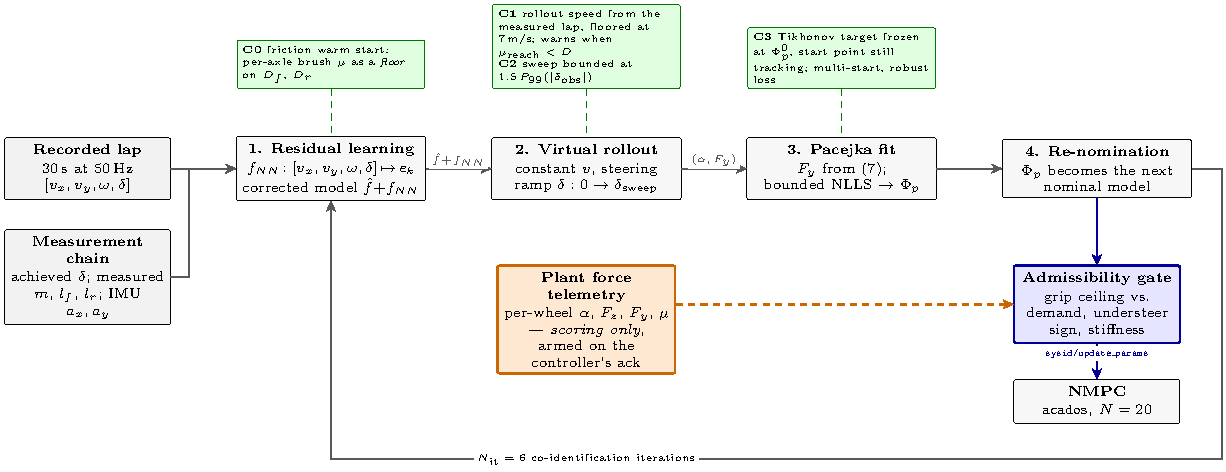
\includegraphics[width=\textheight]{Figures/pipeline.pdf}
\caption{The identification pipeline. Recorded lap data trains the residual
network, the corrected model is rolled out through a synthetic steering sweep,
Pacejka coefficients are fitted to that sweep, and the fit becomes the next
nominal model under relaxation. Green marks this paper's changes: the friction
warm start (Section~\ref{subsec:friction}), the excitation-aware rollout speed
and extrapolation-bounded sweep
(Sections~\ref{subsec:excitation}--\ref{subsec:iterative}), the frozen
regularisation target of Eq.~\eqref{eq:fitobj} and the relaxed update of
Eq.~\eqref{eq:relax}. Blue is the gated controller interface
(Section~\ref{sec:integration}); orange is the plant's per-wheel force
telemetry, which scores the result and never enters the loop.}
\label{fig:pipeline}
\end{sidewaysfigure}

\begin{algorithm}[htbp]
\footnotesize
\caption{Corrected on-track identification cycle. $\triangleright$ marks a
change to the inherited pipeline~\cite{ontrack2025}.}
\label{alg:loop}
\hrule\vspace{2pt}
\algline{in}{buffer $\mathcal{D}=\{v_{x},v_{y},\omega,\delta^{\mathrm{ach}}\}_{1:K}$ ($\SI{30}{\second}$), prior $\phip^{0}$, bounds $[\phip^{-},\phip^{+}]$}
\algline{out}{$\phip$, or \textsc{unidentified}}
\vspace{2pt}\hrule\vspace{2pt}
\algline{1}{$\delta \leftarrow$ achieved road-wheel angle, command on staleness \hfill$\triangleright$}
\algline{2}{$m,l_{f},l_{r} \leftarrow$ measured static wheel loads \hfill$\triangleright$}
\algline{3}{$\hat\mu_{f} \leftarrow \textsc{BrushFit}(\mathcal{D})$, front axle, released only if gated \hfill$\triangleright$}
\algline{4}{\textbf{if} released \textbf{then} $D^{0}_{f},D^{0}_{r} \leftarrow \hat\mu_{f}$; $D$ held for the whole loop \hfill$\triangleright$}
\algline{5}{$\phip^{\mathrm{tik}} \leftarrow \phip^{0}$ \quad(frozen for all iterations) \hfill$\triangleright$}
\algline{6}{$v \leftarrow \mathrm{clip}(\overline{v_{x}}(\mathcal{D}),\,v_{\min},\,\infty)$ \hfill$\triangleright$}
\algline{7}{$\delta_{\mathrm{sweep}} \leftarrow \mathrm{clip}(1.5\,P_{99}(|\delta|),\,\delta_{\min},\,\delta_{\max})$ \hfill$\triangleright$}
\algline{8}{$\mu_{\mathrm{reach}} \leftarrow v^{2}\delta_{\mathrm{sweep}}/(gL)$; \textbf{warn if} $\mu_{\mathrm{reach}}<\max_{a} D^{0}_{a}$ \hfill$\triangleright$}
\algline{9}{$\phip \leftarrow \phip^{0}$; \textbf{for} $i=1$ \textbf{to} $N_{\mathrm{it}}$ \textbf{do}}
\algline{10}{\algin{1.5}$f_{NN} \leftarrow \textsc{TrainResidual}(\mathcal{D},\phip)$; $\mathcal{S} \leftarrow \textsc{Rollout}(\phip,f_{NN},v,\delta_{\mathrm{sweep}})$}
\algline{11}{\algin{1.5}$\tilde\phip \leftarrow \arg\min_{B,C,E}\|F_{y}(\phip;\mathcal{S})-\hat F_{y}(\mathcal{S})\|^{2}+\lambda\|\phip-\phip^{\mathrm{tik}}\|^{2}$, $D$ held \hfill$\triangleright$}
\algline{12}{\algin{1.5}$\phip \leftarrow (1-\beta)\,\phip + \beta\,\tilde\phip$ \quad($\beta=\num{0.20}$) \hfill$\triangleright$}
\algline{13}{\textbf{if} any $\phip$ component on a bound \textbf{then} report the degeneracy \hfill$\triangleright$}
\algline{14}{\textbf{if not} \textsc{Gates}$(\phip)$ \textbf{then return} \textsc{unidentified} \hfill$\triangleright$}
\algline{15}{submit $\phip$; keep the previous model until acknowledged \hfill$\triangleright$}
\vspace{2pt}\hrule\vspace{2pt}
\algline{}{\textsc{Gates}: axle stiffness sign and magnitude; $l_{f}C_{f}<l_{r}C_{r}$ and $v_{\mathrm{crit}}$ outside the speed range; grip ceiling $\ge$ the trajectory's lateral demand (Section~\ref{sec:integration}).}
\end{algorithm}

\subsection{Residual model and objective}
\label{subsec:physinputs}

The residual carries whatever the nominal model
Eqs.~\eqref{eq:vydot}--\eqref{eq:mf} does not represent. The default is the baseline
multilayer perceptron: 4 inputs, one hidden layer of 8 units, 2 outputs,
LeakyReLU, 58 parameters, full-batch Adam~\cite{kingma2015adam} at
$5\times10^{-4}$ on an MSE objective, in PyTorch~\cite{paszke2019pytorch}. The
architecture is selectable; the two arms of Section~\ref{sec:results} use
\texttt{baseline} and \texttt{s4}, the latter an S4D diagonal state-space
residual~\cite{gu2022s4d} over a sliding window of $W=20$ samples
(\SI{0.7}{\second}), so the residual can carry tire-relaxation and yaw-damping
dynamics a per-sample map cannot. We claim neither that architecture, which is
also in concurrent work~\cite{visionsysid2026}, nor the \num{8.7}$\times$
reduction in its training cost, an exact algebraic rewrite that changes no
identified coefficient; both are in the supplementary material, and the
identifiability result below holds for either architecture.

The input space of the \texttt{s4} arm is augmented with the axle slip angles
of Eq.~\eqref{eq:slip}: since the tire law Eq.~\eqref{eq:mf} is a function of
$(\alpha,F_{z})$ and of nothing else, supplying $\alpha_{f},\alpha_{r}$
directly spares the network a relation the model already states. The
augmentation is also available on the MLP, at 16 extra weights
($58\rightarrow74$ parameters), and is off in the \texttt{baseline} arm. The optional physics-informed objective
\begin{equation}
\mathcal{L}=\mathcal{L}_{\mathrm{data}}
+\lambda_{s}\mathcal{L}_{\mathrm{steady}}
+\lambda_{m}\mathcal{L}_{\mathrm{sym}}
+\lambda_{g}\mathcal{L}_{\mathrm{smooth}},
\label{eq:pinnloss}
\end{equation}
with $\lambda_{s}=0.1$, $\lambda_{m}=0.05$, $\lambda_{g}=10^{-4}$, adds three
penalties to the one-step MSE~\cite{raissi2019pinn,deepdynamics2024}:
$\mathcal{L}_{\mathrm{steady}}$ keeps the two residual channels jointly
consistent with Eqs.~\eqref{eq:vydot}--\eqref{eq:omdot} on a quasi-steady mask, so
they cannot imply an axle force pair no tire could produce (stage~3 fits that
force pair, not the state prediction);
$\mathcal{L}_{\mathrm{sym}}$ enforces the odd symmetry $e(-\vecz)=-e(\vecz)$ of
a laterally symmetric vehicle; $\mathcal{L}_{\mathrm{smooth}}$ is a soft
Lipschitz bound.

One property of Eq.~\eqref{eq:pinnloss} is not a hyperparameter.
$\mathcal{L}_{\mathrm{data}}$ is a mean square over a one-step increment while
the two balance residuals are a force and a moment, four to six orders of
magnitude apart, so $\lambda_{s}$ is not a relative weight at all: measured at
initialisation on a \SI{30}{\second} buffer of this vehicle, the unnormalised
steady term contributes \SI{99.9996}{\percent} of $\mathcal{L}$, a ratio of
$\num{2.3}\times10^{5}$, and such a residual fits the nominal model's own force imbalance
instead of the data it was given. Each residual is therefore expressed as the
state increment it implies, the unit the network's output is in,
\begin{equation}
r_{\mathrm{lat}}=\frac{T_{s}}{m}\,\Big(m\dot v_{y}+mv_{x}\omega-(\Fyr+\Fyf\cos\delta)\Big),
\label{eq:physnorm}
\end{equation}
and $r_{\mathrm{yaw}}$ likewise with $T_{s}/I_{z}$. The shares become
\SI{98.53}{\percent} data and \SI{1.47}{\percent} steady, recovering the meaning
Eq.~\eqref{eq:pinnloss} gives $\lambda_{s}$. The weights in Eq.~\eqref{eq:pinnloss} are
relative weights only in these units.

\subsection{Excitation-aware virtual rollout}
\label{subsec:excitation}

Consider stage~2 of
Section~\ref{subsec:baseline}: a constant-speed rollout at $v$ with the steering
ramped to $\delta_{\mathrm{sweep}}$. In quasi-steady cornering the lateral
acceleration a single-track vehicle develops kinematically is
$a_{y}=v^{2}\kappa$ with $\kappa\approx\delta/L$, so the largest friction
coefficient the rollout can \emph{demand} of the tire is
\begin{equation}
\boxed{\;\mu_{\mathrm{reach}}\;\approx\;\frac{v^{2}\,\delta_{\mathrm{sweep}}}{g\,L}\;}
\label{eq:mureach}
\end{equation}
Eq.~\eqref{eq:mureach} contains no tire parameter: it is a property of the
rollout configuration alone, and an \emph{upper} bound rather than an equality,
since the steady-state curvature a compliant vehicle holds is smaller than the
Ackermann $\delta/L$. Reading it as a ceiling is all the argument needs: if even
the ceiling sits below $D$, the synthetic data never leaves the linear ramp of
Eq.~\eqref{eq:mf}, only the product $BCD$ is identifiable
(Section~\ref{subsec:identifiability}), and the bounded optimiser resolves the
residual freedom on a box edge.

The baseline implementation selects the rollout speed as
$v=\mathrm{clip}(\overline{v_{x}},\,2,\,4)\,\si{\meter\per\second}$,
representative of a 1:10 platform. On our vehicle, with
$\delta_{\mathrm{sweep}}=\SI{0.4}{\radian}$ and $L=\SI{1.5334}{\meter}$,
Eq.~\eqref{eq:mureach} gives $\mu_{\mathrm{reach}}=0.43$ at
\SI{4}{\meter\per\second}: the rollout cannot ask the tire for more than
\SI{0.43}{\g} whatever the tire is. At 1:10 scale, with
$L\approx\SI{0.32}{\meter}$, the same speed yields
$\mu_{\mathrm{reach}}\approx2.0$ and the pathology is invisible. The rollout
speed is therefore now taken from the speed the vehicle was actually driven at,
clamped below at \SI{15}{\meter\per\second}, and the pipeline warns whenever
Eq.~\eqref{eq:mureach} evaluates below the prior's $D$, turning a silent degeneracy
into a startup diagnostic. The same bound sets a data-collection requirement:
identification data should be gathered at
$v\ge\sqrt{gLD/\delta_{\mathrm{sweep}}}$.

\subsection{Bounded extrapolation and frozen-prior regularisation}
\label{subsec:iterative}

Raising the rollout speed exposes a second, opposite failure: the rollout
queries the residual network at steering angles it has never seen, the observed
$|\delta|$ on a pure-pursuit lap staying below $\approx\SI{0.06}{\radian}$ while
the sweep ran to \SI{0.4}{\radian}. The fit reads the network's extrapolation as
additional grip, and because each iteration's answer became both the next
iteration's nominal model \emph{and} its regularisation target, the error
compounds: $D$ walked from the \num{1.009}/\num{1.002} prior to
\num{1.5402}/\num{1.8721} over six iterations, a claimed \SI{1.7}{\g} on a
vehicle measuring \SI{1.0}{\g} in steady state.

Two changes close the loop. First, an extrapolation bound: the sweep
terminates at $\delta_{\mathrm{sweep}}=\mathrm{clip}\big(\lambda_{e}
P_{99}(|\delta_{\mathrm{obs}}|),\,\delta_{\min},\,\delta_{\max}\big)$ with
$\lambda_{e}=1.5$, $\delta_{\min}=\SI{0.05}{\radian}$ and
$\delta_{\max}=\SI{0.54}{\radian}$, so the network is never queried more than
\SI{50}{\percent} beyond the steering range it was trained on. Both
$\delta_{\max}$ and the inherited \SI{0.4}{\radian} lie above the plant's
\SI{0.279}{\radian} mechanical lock deliberately: the sweep is a \emph{virtual}
rollout, and clamping it to the lock would cap $\mu_{\mathrm{reach}}$ a second
time, by the actuator instead of the rollout speed
(Appendix~\ref{subsec:assumptions}, A6). Second, a frozen prior: the
Tikhonov target is held at the configured $\phip^{0}$ for all iterations while
the optimiser's \emph{start point} continues to track the previous iteration,
giving the per-axle objective
\begin{equation}
\min_{\phi}\;\sum_{k}\rho\!\big(r_{k}(\phi)\big)\;+\;\sum_{j}w_{j}\big(\phi_{j}-\phi^{0}_{j}\big)^{2},
\label{eq:fitobj}
\end{equation}
with $r_{k}$ the force residual, $\rho$ a soft-$\ell_{1}$ robust loss and
$w_{j}$ scaled to the data residual budget by a single dimensionless weight
$\lambda=0.05$. The regulariser exists to hold the coefficients the manoeuvre
does not excite, $E$ above all, at their nominal value instead of on a box edge.

\subsection{What the rollout fit identifies, and why the loop must be damped}
\label{subsec:contraction}

\subsubsection{The rollout fit sees only the product $BCD$}
\label{subsec:bcd}
In the virtual-data step the low-slip degeneracy of
Section~\ref{subsec:identifiability} is stronger, and structural rather than
excitation-dependent. Stage~3 does not observe a force; it reconstructs one from
the rollout's own quasi-steady yaw balance Eq.~\eqref{eq:ssforces}, which on the
synthetic trajectory reduces to
\begin{equation}
\frac{F_{y,f}}{F_{z,f}}=\frac{v_{x}\omega}{g\cos\delta},\qquad
\frac{F_{y,r}}{F_{z,r}}=\frac{v_{x}\omega}{g},
\label{eq:rollobs}
\end{equation}
so the only quantity Eq.~\eqref{eq:fitobj} ever compares against is the lateral
acceleration the rollout realises, which the \emph{previous} coefficient set
produced through its slope $F_{z}BCD$. The fit's residual therefore
depends on $(B,C,D)$ only through their product, and $D$ is the free coordinate
of the hyperbola $BCD=\mathrm{const}$. Replayed on five identification buffers
of a live $\mu=\num{1.05}$ run, the product is recovered tightly, $BCDF_{z,f}$
over \SIrange{18.9}{21.1}{\kilo\newton\per\radian} against the
\SI{20.4}{\kilo\newton\per\radian} the plant carries at $\bar F_{z}=1$
(Table~\ref{tab:ref}; that run stays below the peak, so the fitted and
closed-form slopes agree there), while the $D$ reaching that same product
ranges over \numrange{0.69}{2.00}. $D$ must therefore not be asked of this fit
at all. It is measured on the \emph{recorded} trace by the brush estimator of
Section~\ref{subsec:friction}, which fits $F_{y}(\alpha)$ directly and is not
subject to Eq.~\eqref{eq:rollobs}, then held fixed while $B$, $C$ and $E$ carry the
stiffness the rollout does determine.

\subsubsection{The loop is not a contraction}
Stage~4 makes each iteration's answer the nominal model stage~2 rolls out, and
stage~3 then fits the trajectory that model produced, over a steering range
already extrapolating $1.5\times$ past the observed one. The fit reads its own
forces back, so the loop is a positive feedback path on its own extrapolation
error rather than a contraction: replayed offline on five recorded buffers, axle
force RMSE against the plant's telemetry degrades monotonically with iteration
count, \num{38.9}, \num{53.0}, \num{58.5} and \SI{70.4}{\newton} at the front
for $N_{\mathrm{it}}\in\{1,2,3,6\}$. Pinning $D$ does not remove this; it
relocates it into $B$, $C$ and $E$. The remedy is to damp the step, not to
shorten the loop, so stage~4 becomes a relaxed fixed-point iteration
\begin{equation}
\phip^{(i)} \leftarrow (1-\beta)\,\phip^{(i-1)} + \beta\,\tilde\phip^{(i)},
\label{eq:relax}
\end{equation}
with $\beta=\num{0.20}$; $\beta=1$ recovers the inherited update exactly. The
sweep over $\beta$ (Section~\ref{subsec:ablations}) carries the control the
contribution needs: $\beta=0$ freezes the coefficients at the pinned prior,
performing no identification at all, and is the worst setting. The iterations do
carry information, but only a damped update preserves it.

Fitting itself applies Eq.~\eqref{eq:ssforces} to the synthetic data under box
constraints $\phip\in([4.0,1.2,0.4,-3.0],[20.0,2.2,2.0,1.0])$ per axle, over
$B$, $C$ and $E$ with $D$ held. Relative to the baseline we raised the jittered
multi-starts from 1 to 8 and added a derivative-free
simplex~\cite{neldermead1965} and a global differential-evolution
solver~\cite{storn1997de} alongside trust-region
reflective~\cite{branch1999trust}, through the same
library~\cite{virtanen2020scipy}. Neither change addresses the degeneracy, and
Section~\ref{subsec:sweep} verifies both as secondary.

\subsection{Measurement-side corrections}
\label{subsec:measurement}

\subsubsection{Achieved steering, measured mass and geometry}
$\alpha_{f}$ in Eq.~\eqref{eq:slip} was built from the \texttt{/drive} setpoint. The
measured achieved/commanded ratio is \num{0.76}, so $\alpha_{f}$ was
systematically $\approx\SI{25}{\percent}$ too large and the fitted front
stiffness $\approx\SI{20}{\percent}$ too small
(\SI{13725}{\newton\per\radian} against \SI{17198}{\newton\per\radian} fitted to
the simulator's own per-wheel forces over the same run); using
\texttt{feedback/\allowbreak steering\_angle} recovers
\SI{18486}{\newton\per\radian}. Separately, $m$ and $l_{wb}$ come from the
measured static wheel loads (Table~\ref{tab:vehicle}) and not a
configuration file, and $l_{wb}\equiv l_{f}+l_{r}$ is enforced by a regression
test, because Eq.~\eqref{eq:ssforces} uses the wheelbase for the normal loads and
the axle split for the force division, and the two disagreeing is a silent bias.

\subsubsection{Proprioceptive friction warm-start}
\label{subsec:friction}
The inherited pipeline had no prior for the peak factor: $D$ started from a
configuration constant and was left to the fit. Newton--Euler on the
single-track body of Eqs.~\eqref{eq:vydot}--\eqref{eq:omdot}, solved for the axle
forces rather than the accelerations, gives
\begin{equation}
F_{y,f}=\frac{I_{z}\dot\omega+l_{r}m a_{y}}{L\cos\delta},\qquad
F_{y,r}=\frac{l_{f}m a_{y}-I_{z}\dot\omega}{L},
\label{eq:newtoneuler}
\end{equation}
which needs the IMU's lateral acceleration and the yaw acceleration and no tire
model; vertical loads carry the longitudinal transfer
$F_{z,f/r}=m(g\,l_{r/f}\mp a_{x}h_{cg})/L$ \cite{rajamani2012}, and yaw
acceleration is the derivative of a local polynomial fit to the yaw rate
(Savitzky--Golay, window 21, order 2)~\cite{savitzky1964} and not a
difference, because $I_{z}\dot\omega$ is a $\approx\SI{10}{\percent}$ term in
$F_{y,f}$ here.

Per axle, cornering stiffness and peak friction are then fitted jointly to the
Fiala brush model~\cite{fiala1954,svendenius2004brush,pacejka2012book}
\begin{equation}
F_{y}=\mu F_{z}\big(1-(1-\xi)^{3}\big)\mathrm{sgn}\,\alpha,\quad
\xi=\min\!\Big(\frac{C_{\alpha}|\tan\alpha|}{3\mu F_{z}},1\Big),
\label{eq:brush}
\end{equation}
by bounded nonlinear least squares with a soft-$\ell_{1}$
loss~\cite{virtanen2020scipy,branch1999trust}, over samples with
$|a_{x}|\le\SI{0.35}{\g}$, the fit being pure-lateral while combined slip
shrinks the lateral capacity~\cite{acosta2017friction}. The brush model
replaces
Eq.~\eqref{eq:mf} here because it has two parameters, both of which the manoeuvre
can support, against the four of the model whose non-identifiability at low slip
this paper is about. What beats the utilisation bound is that $\mu$ enters
Eq.~\eqref{eq:brush} through the \emph{curvature} of $F_{y}(\alpha)$ and not only
through its asymptote: writing $r=|F_{y}|/(C_{\alpha}|\tan\alpha|)$ for the force's
departure from its own linear extrapolation, Eq.~\eqref{eq:brush} inverts to
\begin{equation}
\mu=\frac{2k}{3-\sqrt{3(4r-1)}},\qquad k=\frac{C_{\alpha}|\tan\alpha|}{3F_{z}},
\label{eq:brushinv}
\end{equation}
so a \SI{30}{\percent} departure from linearity ($r=0.7$) already pins $\mu$,
well below the limit.

Eq.~\eqref{eq:brushinv} also states its own failure mode:
$\mathrm{d}\mu/\mathrm{d}r$ grows without bound as the curve stays linear. The
estimate is released only when four conditions hold: absolute grip demand
$\max|F_{y}|/F_{z}\ge\num{0.40}$, peak friction utilisation
$\max|F_{y}|/(\hat\mu F_{z})\ge\num{0.40}$, relative precision
$\sigma_{\hat\mu}/\hat\mu\le\num{0.15}$ from the Gauss--Newton covariance, and
$\hat\mu$ not resting on its own search bound, $[\num{0.2},\num{2.0}]$;
otherwise the module logs which condition failed and falls back to the
utilisation bound. The first two are the
same quantity with and without the fit in the denominator, and both are needed:
the utilisation test divides by the \emph{fitted} $\hat\mu$ of the same
least-squares call, so an axle whose $\mu$ comes out too low clears the gate on
its own error, while the absolute ratio has no such freedom. The
\SI{40}{\percent} floor is the level the friction-estimation literature
converges on~\cite{acosta2017friction}.

\paragraph{Applied two-sided, then pinned}
\label{subsec:frictionfloor}
The released $\hat\mu$ \emph{replaces} $D$ on both axles, in either direction,
and $D$ is then held fixed for the whole co-identification loop. Both axles take
the \emph{front} fit: the rear slip angle does not carry $\delta$, so on this
trajectory the rear force curve has too little curvature to support
Eq.~\eqref{eq:brushinv} and its $\mu$ comes out high
(\num{1.495}/\num{1.383}/\num{1.257} rear against
\num{1.011}/\num{0.964}/\num{0.837} front on three admitted buffers of a
$\mu=\num{1.05}$ run). This is not a yaw-inertia error: in quasi-steady
cornering $F_{y,f}/F_{y,r}\to l_{r}/l_{f}$, the same ratio as
$F_{z,f}/F_{z,r}$, so $\mu_{f}=\mu_{r}$ whatever $I_{z}$ is, and there is one
road surface. It is two-sided and not a floor: the rule it replaces
protected against a $D$ that \emph{moved} between cycles, not against one that
was low; it is pinned and not merely seeded, since Eq.~\eqref{eq:rollobs} leaves $D$
free along $BCD=\mathrm{const}$ and on a live run a \num{0.785} seed ended at
the \num{2.000} bound within one cycle; and an axle with no released $\hat\mu$
holds the $D$ it came in with, since there is nothing in the rollout to fit it
against.

Pinning puts the whole weight of the result on the gate, and $\sigma_{\mu}/\mu$
from the fit covariance is a \emph{precision} figure, not an accuracy one: a
wrong mass, yaw inertia, IMU bias or road bank all fit tightly and wrongly
through Eq.~\eqref{eq:newtoneuler}. Here the configuration file's
\SI{240.0}{\kilo\gram} against the \SI{269.6}{\kilo\gram} the wheels actually
carry biased $\mu$ \SI{11}{\percent} low until the measured value replaced it,
and the configured wheel coefficient is not the effective one the physics step
uses, the server multiplying it by the road surface's \num{0.70}.

\subsection{Deployment and validation protocol}
\label{subsec:deployment}

The identifier runs as a single ROS~2 node cycling a rolling FIFO buffer through
four states (collect, train, await the controller's acknowledgement, run),
re-identifying every $T_{\mathrm{reid}}=\SI{30}{\second}$. Coefficients are
submitted over a service call whose non-acknowledgement leaves the previous
model in place, so a rejected identification degrades to the last accepted model
rather than to none. That acknowledgement also arms the scoring: a submission
the controller \emph{rejects} on its admissibility gate
(Section~\ref{sec:integration}) is a model the car never drove on, and the
seconds between a fit completing and its acknowledgement landing are seconds
still driven on the previous model.

Three levels of validation are used, in increasing strength, and all three score
the \emph{accepted} model only. One-step prediction on a held-out run,
as in the baseline: RMSE and $R^{2}$ of $v_{y}$ and $\omega$, with online
statistics in Welford's form~\cite{welford1962} and samples admitted only above
\SI{1}{\meter\per\second}. Direct force comparison against
\texttt{feedback/\allowbreak tire\_forces}: the identified curve is evaluated at
the measured $(\alpha,F_{z})$ and compared per axle against the measured
$F_{y}$, and against the plant's own curve~Eq.~\eqref{eq:physx} at the same points,
which separates the error of the fit from the error of representing a PhysX
tire. Closed-loop tracking under the MPC: lateral deviation, its
time-weighted integral, heading error and solver cost, split by active
controller so the pure-pursuit acquisition phase is not scored against a model
it does not use.

% === VI. EXPERIMENTS AND RESULTS =============================================
\section{Experiments and Results}
\label{sec:results}

\subsection{Setup}
\label{subsec:setup}

All experiments run on the architecture of Section~\ref{sec:platform}: the
Formula AI vehicle in CARLA driven through ROS~2 Humble, the server in
synchronous mode at a \SI{0.033}{\second} fixed physics step. The identifier
collects \SI{30}{\second} of data on a \SI{50}{\hertz} timer that the server's
step rate holds to \SI{30}{\hertz} (Section~\ref{subsec:data}) and
re-identifies from the newest buffer, matching the baseline's data
budget~\cite{ontrack2025}. Ground truth is the simulator's own per-wheel
telemetry, which the identifier never reads; every figure is exported with the
CSV holding its samples, and the cross-run comparison reads those CSVs rather
than re-deriving any metric.

Two clocks appear below, and no metric mixes them. The controller node stamps
its own quantities (run duration, handover time, lap time and every tracking
error) on the ROS wall clock. The identifier and the force benchmark stamp
theirs on the simulation clock, which the server advances faster than wall time,
at a ratio between \num{1.28} and \num{1.66} across the four runs. Table~\ref{tab:comparison}
labels each block with the clock it is measured on.

\subsubsection{Two friction schedules}
\label{subsubsec:surface}
Four runs are reported, two configurations crossed with two surfaces.

On the \emph{static} surface the per-wheel coefficient is held at its configured
\num{1.0}, and the road-surface factor of \num{0.70} PhysX applies on top of it
makes the effective coefficient \num{0.700}, constant to the last digit the
simulator reports over all force-validation samples of both runs. It is
deliberately not the $\mu=\num{1.05}$ surface the tire prior was measured on
(Section~\ref{subsubsec:priorprovenance}), so an arm that cannot move off its
prior cannot score well. What it does not test is tracking: the identifier is
asked to find one number and then hold it.

The \emph{decaying} surface supplies the change. A schedule node drives the
per-wheel coefficient over the ROS wall clock through
\begin{equation}
\mu_{\mathrm{cmd}}(t)=\max\!\big(\mu_{\mathrm{floor}},\;\mu_{0}(1-\eta t)\big),
\qquad \eta=10^{-3}\,\si{\per\second},
\label{eq:decay}
\end{equation}
with $\mu_{0}=\num{1.0}$ and $\mu_{\mathrm{floor}}=\num{0.5}$, reached at
$t=\SI{500}{\second}$; the command is applied through the bridge's
\texttt{set\_tire\_friction} service while the car is driving, so the surface
changes under a moving vehicle rather than between runs. The effective axle
coefficient the plant reports therefore falls monotonically from \num{0.700} to
the \num{0.350} floor, half the grip gone over the run, and the force-validation
window opens at \num{0.637}. The linear-decay protocol is that of
LLA-MPC~\cite{llampc2025}, which decays $\mu$ at \SI{2}{\percent} of nominal per
second on a 1:43 vehicle. We keep the law and the total excursion and reduce the
rate by a factor of \num{20}, because the scaling of the platform sets what an
on-track identifier can be scored against at all: at \SI{2}{\percent} per second
the surface is exhausted in \SI{50}{\second}, shorter than one
\SI{30}{\second} buffer plus the \SI{20.9}{\second} its fit takes
(Section~\ref{subsec:runtime}), and no identifier of this class would publish a
second coefficient set before the experiment ended. At Eq.~\eqref{eq:decay}'s rate
the surface instead loses about \num{0.06} of $\mu$ per identification cycle,
which is the regime in which tracking is a question rather than a race against
the sampling period.

\subsubsection{Reference trajectory}
\label{subsubsec:raceline}
All four runs follow the same optimised raceline (Figure~\ref{fig:raceline}),
generated with the TUM global race trajectory optimisation
package~\cite{tumracetraj} under its minimum-curvature
formulation~\cite{heilmeier2020}: a closed \SI{5828.2}{\meter} lap of
\num{2916} waypoints, reference speed
\SIrange{9.62}{25.78}{\meter\per\second}, minimum corner radius
\SI{18.7}{\meter} ($|\kappa|_{\max}=\SI{0.0536}{\per\meter}$). Its peak lateral
demand is $\max(v_{x}^{2}|\kappa|)=\SI{4.98}{\meter\per\second\squared}$
(\SI{0.51}{\g}), roughly \SI{73}{\percent} of the \SI{0.70}{\g} the static
surface sustains. On the decaying surface that same trajectory stops being
admissible part way through the run, which is the point of running it: the
plant passes below the reference's demand at an effective $\mu$ of about
\num{0.51}, and what the two arms do about it is the result of
Section~\ref{subsec:resultsclosedloop}.

\subsubsection{The two configurations}
\label{subsubsec:scenarios}
The two configurations of the pipeline differ in the nine settings of
Table~\ref{tab:scenarios} and in nothing else; vehicle, map, trajectory,
controller, data budget, loop count, tire prior and box constraints are shared,
and each configuration meets both surfaces with the same parameter file.
\basearm{} is the inherited configuration evaluated at full scale on the
corrected rollout speed, so the comparison isolates those nine settings rather
than reproducing the published pipeline in full; \oursarm{} is the shipped
configuration. Since the settings move together, what follows is a
configuration comparison, not a per-factor ablation, which
Section~\ref{subsec:ablations} supplies offline for the four that carry the
result. Nor is it a test of this paper's central contribution: the rollout
speed is taken from the measured lap in \emph{both} arms, and no run's mean
speed falls below \SI{16}{\meter\per\second}, so \oursarm{}'s
\SI{15}{\meter\per\second} floor never binds. The excitation correction itself,
together with the operating point it ships, is established in
Section~\ref{subsec:sweep}.

\begin{table}[htbp]
\caption{The two configurations. Each is run on both surfaces.}
\label{tab:scenarios}
\centering
\begin{threeparttable}
\footnotesize
\setlength{\tabcolsep}{4pt}
\begin{tabular}{@{}lll@{}}
\toprule
Setting & \basearm{} & \oursarm{}\\
\midrule
Residual architecture & MLP (\texttt{baseline}) & S4D (\texttt{s4})\\
Residual objective & One-step MSE & Physics-informed,
Eq.~\eqref{eq:pinnloss}\\
Model integrator & Euler & RK4\\
Sweep amplitude & Fixed \SI{0.40}{\radian} & $1.5P_{99}(|\delta|)$, clipped\\
Pacejka solver & Trust-region~\cite{branch1999trust} & Differential
evolution~\cite{storn1997de}\\
Tikhonov weight $\lambda$ & \num{0} & \num{0.05}, frozen target\\
Friction warm start & Off & On; $D$ pinned per axle\\
Fast-$\mu$ derate & Off & On, \SI{1}{\hertz} on \SI{6}{\second}\\
Update relaxation $\beta$ & \num{1.00} (undamped) & \num{0.20}\\
\bottomrule
\end{tabular}
\begin{tablenotes}[flushleft]\scriptsize
\item Everything not listed is identical between the two, the tire prior and
the box constraints included. $\beta$ is the relaxation of Eq.~\eqref{eq:relax};
\num{1.00} is the inherited undamped update. The fast-$\mu$ derate is the brush
estimator of Section~\ref{subsec:friction} refitted on a trailing
\SI{6}{\second} window between coefficient cycles and published as an optional
ratio the controller applies to the identified grip ceiling, clamped to
$[\num{0.4},\num{1.2}]$; with the warm start off there is nothing to publish.
The rollout speed is taken from the measured lap in both arms and is not a
difference here.
\end{tablenotes}
\end{threeparttable}
\end{table}

\subsubsection{Provenance of the tire prior}
\label{subsubsec:priorprovenance}
The prior $\phip^{0}$ both arms start from, and that the Tikhonov term of
Eq.~\eqref{eq:fitobj} pulls toward, is the measured tire of Table~\ref{tab:ref},
obtained by fitting Eq.~\eqref{eq:mf} to CARLA's own per-wheel telemetry over a
dedicated limit-excitation run that reached $\alpha=\SI{0.37}{\radian}$, axle
$\mu=\num{1.05}$ and \SI{1.50}{\g}. It is not independent of the validation
data, and the manoeuvre that produced it is one the pipeline is not allowed to
run, the raceline peaking at \SI{0.51}{\g}. Decisively, it was measured on a
surface none of these runs use, carrying $D=\num{1.009}/\num{1.002}$ and axle
slopes of \num{13.2} and \SI{13.9}{\kilo\newton\per\radian} against the
\num{0.70} and the \num{17.4} and \SI{16.6}{\kilo\newton\per\radian} the static
surface realises. Returning it unchanged is a \SI{44}{\percent} grip
overstatement on the static surface and a \SI{188}{\percent} one at the
decaying surface's floor, so an arm has to move away from that prior, in the
right direction, to score well, and on the decaying surface it has to keep
moving.

\subsection{Selecting the rollout operating point $(v,\delta_{\mathrm{sweep}})$}
\label{subsec:sweep}

This grid is where the rollout configuration the pipeline ships is
\emph{chosen}: the
\SI{15}{\meter\per\second} speed floor and the
$\delta_{\max}=\SI{0.54}{\radian}$ clip of Section~\ref{subsec:excitation} are
read off Table~\ref{tab:sweep}, and the reachable-friction bound
Eq.~\eqref{eq:mureach} is what makes the search one-dimensional instead of a blind
scan. The search is run where the answer is known exactly and not in CARLA,
since a CARLA lap cannot be scored against a $D$ nobody knows. A tire with a
known peak factor $D$ is rolled out through the synthetic sweep of stage~2 (the
shipped rollout, residual network set to zero) and fitted back with the shipped
solver, \emph{unregularised} and started from the true coefficients, so
everything it loses is lost to excitation. Rollout speed $v$, sweep amplitude
$\delta_{\mathrm{sweep}}$ and true $D$ are swept, each cell repeated over five
noise realisations at the one-step persistence RMSE measured on CARLA runs of
this vehicle. The configuration axes are swept one at a time, because
$\mu_{\mathrm{reach}}$ is a function of both. The selection criterion is the one
the pipeline needs: the widest range of true $D$ recovered without railing, over
the whole \numrange{0.70}{1.80} column span, since the tire is unknown when the
configuration is fixed. The span matters twice over on a decaying surface, where
one configuration has to cover every $D$ the run passes through.

\begin{table}[htbp]
\caption{The search that fixes the shipped rollout operating point: peak factor
$\hat D$ recovered from a known tire, swept along both arguments of
$\mu_{\mathrm{reach}}$. The shipped $(v,\delta_{\mathrm{sweep}})$ is selected
from this grid.}
\label{tab:sweep}
\centering
\begin{threeparttable}
\footnotesize
\setlength{\tabcolsep}{6pt}
\begin{tabular}{@{}rrcccc@{}}
\toprule
swept & $\mu_{\mathrm{reach}}$ & \multicolumn{4}{c}{$\hat D$ (railed of 8) at true $D$ of}\\
\cmidrule(l){3-6}
value & & 0.70 & 1.05 & 1.40 & 1.80\\
\midrule
\multicolumn{6}{@{}l}{\emph{(a) rollout speed $v$ [\si{\meter\per\second}] swept at $\delta_{\mathrm{sweep}}=\SI{0.40}{\radian}$}}\\
4 & 0.43 & \num{0.52}$\pm$\num{0.036} (1.8) & \num{0.57}$\pm$\num{0.013} (2.8) & \num{0.59}$\pm$\num{0.018} (3.8) & \num{0.50}$\pm$\num{0.001} (7)\\
6 & 0.96 & \num{0.68}$\pm$\num{0.001} (1) & \num{1.04}$\pm$\num{0.014} (1.2) & \num{1.22}$\pm$\num{0.066} (1.8) & \num{1.26}$\pm$\num{0.097} (2)\\
8 & 1.70 & \num{0.69}$\pm$\num{0.001} (1) & \num{1.02}$\pm$\num{0.001} (0.8) & \num{1.36}$\pm$\num{0.002} (0) & \num{1.79}$\pm$\num{0.025} (1.2)\\
13 & 4.49 & \num{0.72}$\pm$\num{0.001} (0) & \num{1.05}$\pm$\num{0.002} (0) & \num{1.38}$\pm$\num{0.001} (0.4) & \num{1.77}$\pm$\num{0.002} (0.4)\\
20 & 10.64 & \num{0.92}$\pm$\num{0.004} (1) & \num{1.14}$\pm$\num{0.005} (0.4) & \num{1.43}$\pm$\num{0.002} (0) & \num{1.80}$\pm$\num{0.005} (0)\\
\addlinespace
\multicolumn{6}{@{}l}{\emph{(b) $\delta_{\mathrm{sweep}}$ [\si{\radian}] swept at $v=\SI{15}{\meter\per\second}$}}\\
0.03 & 0.45 & \num{0.80}$\pm$\num{0.019} (2) & \num{1.10}$\pm$\num{0.041} (2) & \num{1.08}$\pm$\num{0.182} (2) & \num{1.09}$\pm$\num{0.397} (2)\\
0.06 & 0.90 & \num{0.92}$\pm$\num{0.003} (2) & \num{1.30}$\pm$\num{0.008} (2) & \num{1.68}$\pm$\num{0.017} (2) & \num{1.80}$\pm$\num{0.232} (3.4)\\
0.15 & 2.24 & \num{0.99}$\pm$\num{0.004} (2) & \num{1.38}$\pm$\num{0.003} (2) & \num{1.71}$\pm$\num{0.019} (2) & \num{1.98}$\pm$\num{0.009} (1)\\
0.40 & 5.98 & \num{0.76}$\pm$\num{0.009} (1) & \num{1.05}$\pm$\num{0.002} (0) & \num{1.39}$\pm$\num{0.002} (0) & \num{1.78}$\pm$\num{0.001} (0)\\
0.54 & 8.08 & \num{0.83}$\pm$\num{0.004} (1) & \num{1.08}$\pm$\num{0.002} (0) & \num{1.38}$\pm$\num{0.001} (0) & \num{1.78}$\pm$\num{0.008} (0)\\
\bottomrule
\end{tabular}
\begin{tablenotes}[flushleft]\scriptsize
\item Unregularised, started from the true coefficients. Each cell is $\hat D$ $\pm$ the half-width of its \SI{95}{\percent} $t$-interval over five noise realisations, with the mean number of the eight coefficients resting on a box constraint in parentheses. The two axles of one rollout are not independent, so each realisation contributes the mean of its own $(\hat D_{f},\hat D_{r})$ and $n=5$.
\item $\mu_{\mathrm{reach}}$ is Eq.~\eqref{eq:mureach} at $L=\SI{1.5334}{\meter}$; the inherited configuration is the first row of (a). It is the Ackermann \emph{upper} bound and above $\mu_{\mathrm{reach}}\approx2$ detaches from what the rollout realises, so a large value means ``far past saturation'', not a demand the tire ever sees.
\end{tablenotes}
\end{threeparttable}
\end{table}

The grid says three things. First, the inherited \SI{4}{\meter\per\second}
rollout is uninformative about $D$ at \emph{every} grip level tested: the
$0.70$, $1.05$, $1.40$ and $1.80$ tires all come back as $\hat D$ between
\num{0.50} and \num{0.59}, with two to seven of the eight coefficients on a
bound, so the fit reports $\mu_{\mathrm{reach}}$ and not the tire. Second, the
boundary is $\mu_{\mathrm{reach}}\gtrsim D$ and not a speed: at
\SI{6}{\meter\per\second}, where $\mu_{\mathrm{reach}}=0.96$, the $0.70$ and
$1.05$ tires are recovered to within \SI{3}{\percent} while the $1.40$ and
$1.80$ tires are \SI{13}{\percent} and \SI{30}{\percent} short, and for
$\mu_{\mathrm{reach}}$ between \num{1.7} and \num{4.5} every tire is recovered
to within \SI{4}{\percent} with no systematic railing. Nor is the bound a
quantity to maximise: at $v=\SI{20}{\meter\per\second}$,
$\mu_{\mathrm{reach}}=\num{10.64}$, the rollout sits far past saturation for
every tire on the grid and $\hat D$ re-biases upward, the \num{0.70} tire
returning \num{0.92}. Third, the failure is not the solver's: multi-start, a
global solver or a better start point cannot recover a coefficient the data
does not contain.

Panel (b) sweeps the other argument of Eq.~\eqref{eq:mureach}. Starving the
amplitude destroys $D$ just as starving the speed does, so speed is not the
governing variable, and the rollout rather than the tire sets the direction of
the error: an under-speeded rollout returns \emph{too little} grip, an
under-swept one too much (at $\delta_{\mathrm{sweep}}=\SI{0.06}{\radian}$ the
\num{1.05} tire comes back at \num{1.30} and the \num{1.40} tire at \num{1.68},
two of the eight coefficients on a bound throughout those rows). That is the
signature of an unidentified parameter, not a biased one. The axes do
\emph{not} collapse onto a common $\mu_{\mathrm{reach}}$, for the upper-bound
reason of Section~\ref{subsec:excitation}: at $v=\SI{20}{\meter\per\second}$
Eq.~\eqref{eq:mureach} reads \num{10.64} against a realised
\numrange{1.40}{2.18}. Read against the realised demand both axes behave alike,
so Eq.~\eqref{eq:mureach} is a cheap screening bound, conclusive when it falls
below $D$, and not a measure of excitation achieved.

The two panels fix the shipped point between a lower edge and an upper one. On
speed, railing loses the \num{1.40} and \num{1.80} tires at
$v\le\SI{6}{\meter\per\second}$ and the saturation re-bias spoils the
\num{0.70} tire at \SI{20}{\meter\per\second}; only $v=\num{8}$ and
$v=\num{13}$ recover every tire in the span to within \SI{4}{\percent}, and the
\SI{15}{\meter\per\second} floor sits inside that band with the measured lap
speed governing above it. On amplitude,
$\delta_{\mathrm{sweep}}\le\SI{0.15}{\radian}$ holds two coefficients on a
bound at every $D$, while \SI{0.40}{\radian} and \SI{0.54}{\radian} rail
nothing, so \SI{0.54}{\radian} is taken as $\delta_{\max}$, the ceiling of the
$1.5P_{99}$ clip that selects the amplitude on a given lap. All of it is a best
case: with the residual set to zero a Magic Formula is fitted to Magic-Formula
data under exactly matched structure, so the selected point is the best setting
\emph{on this grid} and not a proven optimum.

\subsection{Cross-run summary}
\label{subsec:summary}

Table~\ref{tab:comparison} is the complete comparison over both surfaces. On
the static surface \oursarm{} is better on every quantity scored against the
plant and behind only on QP solve time, by \SI{5}{\percent} of the RMS and
\SI{1}{\percent} of the worst case, both two orders of magnitude inside the
control period. The margins are \numrange{9.0}{12.1}$\times$ on peak friction
and axle force and \num{1.5}$\times$ on MPC tracking error.

On the decaying surface the comparison stops being a margin and becomes an
outcome. \oursarm{} completes the same three timed laps, at
\SI{0.139}{\meter} RMS lateral error under MPC, which is its static-surface
figure to within \SI{8}{\percent} although half the grip is gone by the end.
\basearm{} leaves the track in lap~2 and the run is scored as a failure, its
\SI{23.7}{\meter} RMS error under MPC being the departure itself rather than a
tracking quality. The peak-friction column is where the two diverge first:
\oursarm{} follows the surface down, \basearm{} publishes $D=\num{2.000}$
throughout, and the \num{1.408} error that implies is what the controller is
holding when the trajectory stops being admissible. The rest of this section
reads those rows against the figures; Section~\ref{subsec:ablations} attributes
them.

% Too wide for the text block at any readable size, so it is rotated, as the
% template's guidance for a long table asks.
\begin{sidewaystable}
\caption{Cross-run comparison. Two configurations on two surfaces.}
\label{tab:comparison}
\centering
\begin{threeparttable}
\footnotesize
\setlength{\tabcolsep}{5pt}
\begin{tabular}{@{}lrrrr@{}}
\toprule
& \multicolumn{2}{c}{Static surface, $\mu=0.700$} & \multicolumn{2}{c}{Decaying surface, $\mu:0.700\rightarrow0.350$}\\
\cmidrule(lr){2-3}\cmidrule(l){4-5}
Metric & \oursarm{} & \basearm{} & \oursarm{} & \basearm{}\\
\midrule
\multicolumn{5}{@{}l}{\emph{Outcome and closed-loop tracking (wall clock)}}\\
Timed laps completed & \textbf{3} & \textbf{3} & \textbf{3} & 1 (off track, lap 2)\\
Run duration [\si{\second}] & 580.4 & 554.6 & 640.9 & 358.7\\
Lap times [\si{\second}] & 175.2 / 145.4 / 142.8 & 162.3 / 135.8 / 138.0 & 189.8 / 160.9 / 169.2 & 167.7 / --- / ---\\
RMS $e_{y}$, overall [\si{\meter}] & \textbf{0.256} & 0.319 & \textbf{0.264} & 21.505\\
RMS $e_{y}$, MPC [\si{\meter}] & \textbf{0.151} & 0.224 & \textbf{0.139} & 23.705\\
Max $|e_{y}|$, MPC [\si{\meter}] & \textbf{0.683} & 0.776 & \textbf{0.664} & 38.386\\
ITAE $e_{y}$, MPC [\si{\meter\second\squared}] & \textbf{15925} & 25384 & \textbf{17888} & $1.32\times10^{6}$\\
MPC solve, RMS / max [\si{\milli\second}] & 0.399 / 2.604 & \textbf{0.380 / 2.568} & \textbf{0.420 / 3.589} & 0.678 / 4.062\\
\addlinespace
\multicolumn{5}{@{}l}{\emph{Axle lateral force against per-wheel telemetry (simulation clock)}}\\
Front / rear RMSE [\si{\newton}] & \textbf{27.2 / 33.2} & 329.6 / 348.4 & \textbf{32.9 / 36.5} & 171.4 / 178.3\\
Front / rear $R^{2}$ & \textbf{0.993 / 0.987} & $-0.160$ / $-0.461$ & \textbf{0.984 / 0.977} & 0.708 / 0.647\\
Front / rear max abs.\ error [\si{\newton}] & \textbf{264 / 135} & 1295 / 1316 & \textbf{249 / 236} & 2507 / 2069\\
\addlinespace
\multicolumn{5}{@{}l}{\emph{Peak friction against the plant's effective $\mu$}}\\
Front / rear $\mu$ RMSE, whole run & \textbf{0.145 / 0.142} & 1.300 / 1.300 & \textbf{0.209 / 0.207} & 1.408 / 1.408\\
Front / rear $\mu$ RMSE, after release & \textbf{0.078 / 0.078} & 1.300 / 1.300 & \textbf{0.149 / 0.149} & 1.408 / 1.408\\
\addlinespace
\multicolumn{5}{@{}l}{\emph{One-step state prediction}}\\
$v_{y}$ / $\omega$ RMSE [\si{\meter\per\second}, \si{\radian\per\second}] & \textbf{0.014 / 0.049} & 0.156 / 0.104 & \textbf{0.011 / 0.037} & 0.055 / 0.105\\
\addlinespace
\multicolumn{5}{@{}l}{\emph{Last accepted coefficient set, front / rear}}\\
$B$ & 12.89 / 13.75 & 7.64 / 11.19 & 16.10 / 16.42 & \textbf{4.00} / \textbf{4.00}\\
$C$ & 1.240 / 1.248 & 1.806 / 1.346 & 1.362 / 1.416 & 1.204 / 1.591\\
$D$ & 0.768 / 0.768 & \textbf{2.000} / \textbf{2.000} & 0.460 / 0.460 & \textbf{2.000} / \textbf{2.000}\\
$E$ & $-2.52$ / $-1.84$ & \textbf{$-3.00$} / $-1.77$ & $-2.08$ / $-1.40$ & \textbf{$-3.00$} / $-1.74$\\
Axle stiffness [\si{\kilo\newton\per\radian}] & 16.9 / 16.8 & 37.9 / 38.4 & 13.8 / 13.6 & 13.2 / 16.2\\
Grip ceiling Eq.~\eqref{eq:gripceiling} [\si{\g}] & 0.77 & 2.00 & 0.46 & 2.00\\
Plant grip at that moment [\si{\g}] & 0.70 & 0.70 & 0.35 & 0.53\\
\bottomrule
\end{tabular}
\begin{tablenotes}[flushleft]\scriptsize
\item Bold marks the better arm within a surface for the metric blocks, and a
coefficient resting on a box constraint in the coefficient block. The box is
$\phip\in([4.0,1.2,0.4,-3.0],[20.0,2.2,2.0,1.0])$ per axle. The \basearm{}
decaying-surface row is the last set it published before leaving the track, and
its tracking figures are the departure, not a tracking quality. Lap times run on
the ROS wall clock while the simulator advances its fixed step faster than real
time, at a ratio that differs between runs, so they are not read as a
vehicle-performance comparison across arms; within the \oursarm{} column the
static-to-decaying difference is discussed in
Section~\ref{subsec:resultsclosedloop}.
\end{tablenotes}
\end{threeparttable}
\end{sidewaystable}

\subsection{Identified tire model}
\label{subsec:resultstire}

The coefficient block of Table~\ref{tab:comparison} separates the two arms
before any downstream metric does.

First, no coefficient of \oursarm{} rests on a box constraint in any accepted
identification of either run. \basearm{} puts $D$ on its upper bound of
\num{2.000} on both axles in \emph{every} accepted identification of both runs
and $E_{f}$ on its lower bound of \num{-3.0} likewise, and on the decaying
surface it adds $B$ on its lower bound of \num{4.0} on both axles, so five of
its eight coefficients are resting on an edge in the set the car was driving on
when it left the track. The \emph{inner} fits are a separate matter:
\oursarm{}'s static run logs \num{35} fits that stopped on a bound, \num{30} of
them on $C$'s lower \num{1.2} and none on $D$, which the pin takes out of the
fit, against \num{96} for \basearm{} spread over $B$, $C$ and $D$; on the
decaying surface the count rises to \num{56}, still concentrated on $C$. It is the
relaxation of Eq.~\eqref{eq:relax} that keeps the accepted set off an edge its
iterates touch. A peak factor of \num{2.000} against a plant realising
\num{0.700} is less a \SI{186}{\percent} parameter error than the box-edge
signature of Section~\ref{subsec:identifiability}: the coefficient is not
identified, and no per-coefficient bounds check distinguishes that from a fit.

Second, the linear range is identified rather than inherited. Every stiffness in
the table is Eq.~\eqref{eq:stiffness} at the static axle loads
$F_{z,f}=\SI{1373}{\newton}$, $F_{z,r}=\SI{1274}{\newton}$; for the plant it is
the slope fitted to the simulator's own per-wheel forces over
$|\alpha|\in[\num{0.005},\num{0.02}]\,\si{\radian}$, so the two are comparable.
The static surface realises \SI{17.4}{\kilo\newton\per\radian} front and
\SI{16.6}{\kilo\newton\per\radian} rear over this run's load range, below the
$\bar F_{z}=1$ closed-form values of Table~\ref{tab:ref} for the reason its
first footnote gives. The prior carries \num{13.2} and \num{13.9},
\SI{24}{\percent} and \SI{16}{\percent} low; \oursarm{} returns \num{16.9} and
\num{16.8}, \SI{3.2}{\percent} low front and \SI{1.4}{\percent} high rear,
removing \SI{87}{\percent} and \SI{91}{\percent} of the prior's error, and the
product $BCDF_{z}$ that the rollout fit determines
(Section~\ref{subsec:bcd}) then holds within
\SIrange{16.0}{16.9}{\kilo\newton\per\radian} over the five cycles after the
gate releases. \basearm{} returns \num{37.9} and \num{38.4},
\SI{118}{\percent} and \SI{132}{\percent} high, which is $D=\num{2.0}$
multiplying a $B$ the fit chose against it. On the decaying surface
\oursarm{}'s stiffness falls with the surface, to \num{13.8} and
\SI{13.6}{\kilo\newton\per\radian} at the last accepted set, while \basearm{}
arrives at \num{13.2} and \SI{16.2}{\kilo\newton\per\radian} by a different
route: $B$ at its floor multiplied by $D$ at its ceiling. A plausible stiffness
assembled from two railed coefficients is the clearest case this paper has for
gating on derived quantities rather than on coefficients, since the stiffness
gate passes it.

Third, both sets keep the understeer sign and pass the stability gate of
Section~\ref{subsec:gates}; what separates them is the grip ceiling, which
Eq.~\eqref{eq:gripceiling} puts at \SI{2.00}{\g} for \basearm{} on both surfaces
against \SI{0.77}{\g} and \SI{0.46}{\g} for \oursarm{}. The baseline's ceiling
is a claim the plant cannot honour by a factor of \num{2.8} on the static
surface and \num{3.8} at the moment the car leaves the decaying one, and the
grip gate is one-sided, so it passes both. All of these readings are possible
because the lap traverses part of the curvature:
$P_{99}(|\alpha|)=\SI{2.7}{\degree}$ and $\max|\alpha|=\SI{5.8}{\degree}$
against the \SI{8.0}{\degree} at which the plant's curve peaks on the static
surface, and $\max|F_{y}|/F_{z}$ reaches \num{0.71} front and \num{0.72} rear
in transients against \num{0.49} and \num{0.50} at $P_{99}$. This is not a
limit manoeuvre, but it suffices for the friction gate to release, which on the
$\mu=\num{1.05}$ runs it did not; as the decaying surface falls the same lap
becomes relatively more demanding, so the gate keeps releasing rather than
closing.

\subsection{Peak friction: holding one surface, tracking another}
\label{subsec:resultsmu}

Figures~\ref{fig:mutimeseries} and~\ref{fig:mutimeseriesdecay} show what each
arm published for the peak factor over the two runs, and Table~\ref{tab:comparison} gives the errors behind it. The
pinned-$D$ design of Section~\ref{subsec:friction} is directly observable here,
because both arms start \SI{44}{\percent} away from the static answer and
\SI{188}{\percent} away from the decaying one's floor.

On the static surface \oursarm{} publishes six accepted identifications. The
first carries $D_{f}=\num{1.009}$, $D_{r}=\num{1.002}$: the friction gate
rejected that buffer, so the axles held the prior they came in with, the
hold-rather-than-fit rule of Section~\ref{subsec:frictionfloor} and not a fitted
value. From $t=\SI{140.6}{\second}$ the gate releases on every subsequent cycle
and the published peak factor drops to \num{0.779}, \num{0.821}, \num{0.749},
\num{0.756} and \num{0.768}, front and rear alike, against a plant at
\num{0.700}: \SI{10.7}{\percent} high on average, from a prior that was
\SI{44}{\percent} high. The whole-run $\mu$ RMSE is dominated by the first
\SI{140}{\second} at the prior; after the first release it is \num{0.078} on
both axles.

On the decaying surface the same six cycles land on a surface that has moved
between each of them. The gate again rejects the first buffer and releases from
$t=\SI{145.1}{\second}$, and the published peak factor then falls monotonically:
\num{0.706}, \num{0.679}, \num{0.609}, \num{0.525} and \num{0.460}, against a
plant falling from \num{0.580} to \num{0.350} over the same interval. Read as a
rate, the identifier recovers the decay itself: the published sequence falls at
$4.28\times10^{-4}\,\si{\per\second}$ against the plant's
$4.00\times10^{-4}\,\si{\per\second}$, a
\SI{7}{\percent} error on the quantity that a static surface cannot test at all.
Read as a level it carries two offsets, and separating them matters. Each cycle
is fitted on the buffer that preceded it, so the published value describes the
surface of roughly one cycle earlier; against the plant one cycle back the
residual is \SIrange{10.9}{17.4}{\percent} high, mean \SI{14.3}{\percent},
against the \SI{10.7}{\percent} the same estimator carries on a surface that
does not move. The apparent whole-run RMSE of \num{0.209} is therefore that
familiar brush-model bias plus one cycle of transport lag on a surface losing
about \num{0.06} of $\mu$ per cycle, and not a new error mode. The remedy for
the lag is a shorter cycle rather than a better fit, and the fast-$\mu$ derate
of Table~\ref{tab:scenarios} is that shorter cycle; on this run it spent the
last cycles at the upper end of its clamp and so did not shorten anything
(Section~\ref{subsec:ablations}).

\basearm{} returns $D=\num{2.000}$ on both axles in every accepted
identification of both runs and never leaves the bound. On the static surface
that is a constant $\mu$ error of \num{1.300}, so \oursarm{} is
\num{9.0}$\times$ better on the whole-run figure and \num{16.7}$\times$ better
once its warm start has released. On the decaying surface the error grows as
the plant walks away from the bound, reaching \num{1.408} RMSE before the run
ends early, and \oursarm{} is \num{6.7}$\times$ better there. Two
qualifications belong on this whole subsection: the peak factor is
\emph{measured} by the brush estimator on the recorded trace and then held, not
recovered by the Pacejka fit, which Section~\ref{subsec:bcd} shows cannot
recover it; and the residual bias is one-signed, consistent with the brush
model's tendency to over-read $\mu$ where the curve is not fully traversed,
which is also why the tracking result below has margin to work with.
Appendix~\ref{subsec:mu} evaluates the same estimator on a synthetic brush-tire
plant, where $\mu$ is known exactly and the excitation can be swept
independently of it, and shows that it is flat in excitation above its gate
while the utilisation bound it replaces is not.

\begin{figure}[htbp]
\centering
% Front-axle column only: the rear panels are numerically identical (D is pinned
% to the same value on both axles), so they are cropped to give the front panels
% the full width. Trim is in PDF points on the 864x460.8 pt page shared by both
% files; the gutter between the two panel columns sits at x = 652..669 px of a
% 1320 px raster, and the top 40 px carry the now-redundant suptitle. The bottom
% 25 pt are the strip Comparison.save reserves in both files for the
% incomplete-run banner, which the right trim would otherwise slice mid-word;
% the caption states the same fact.
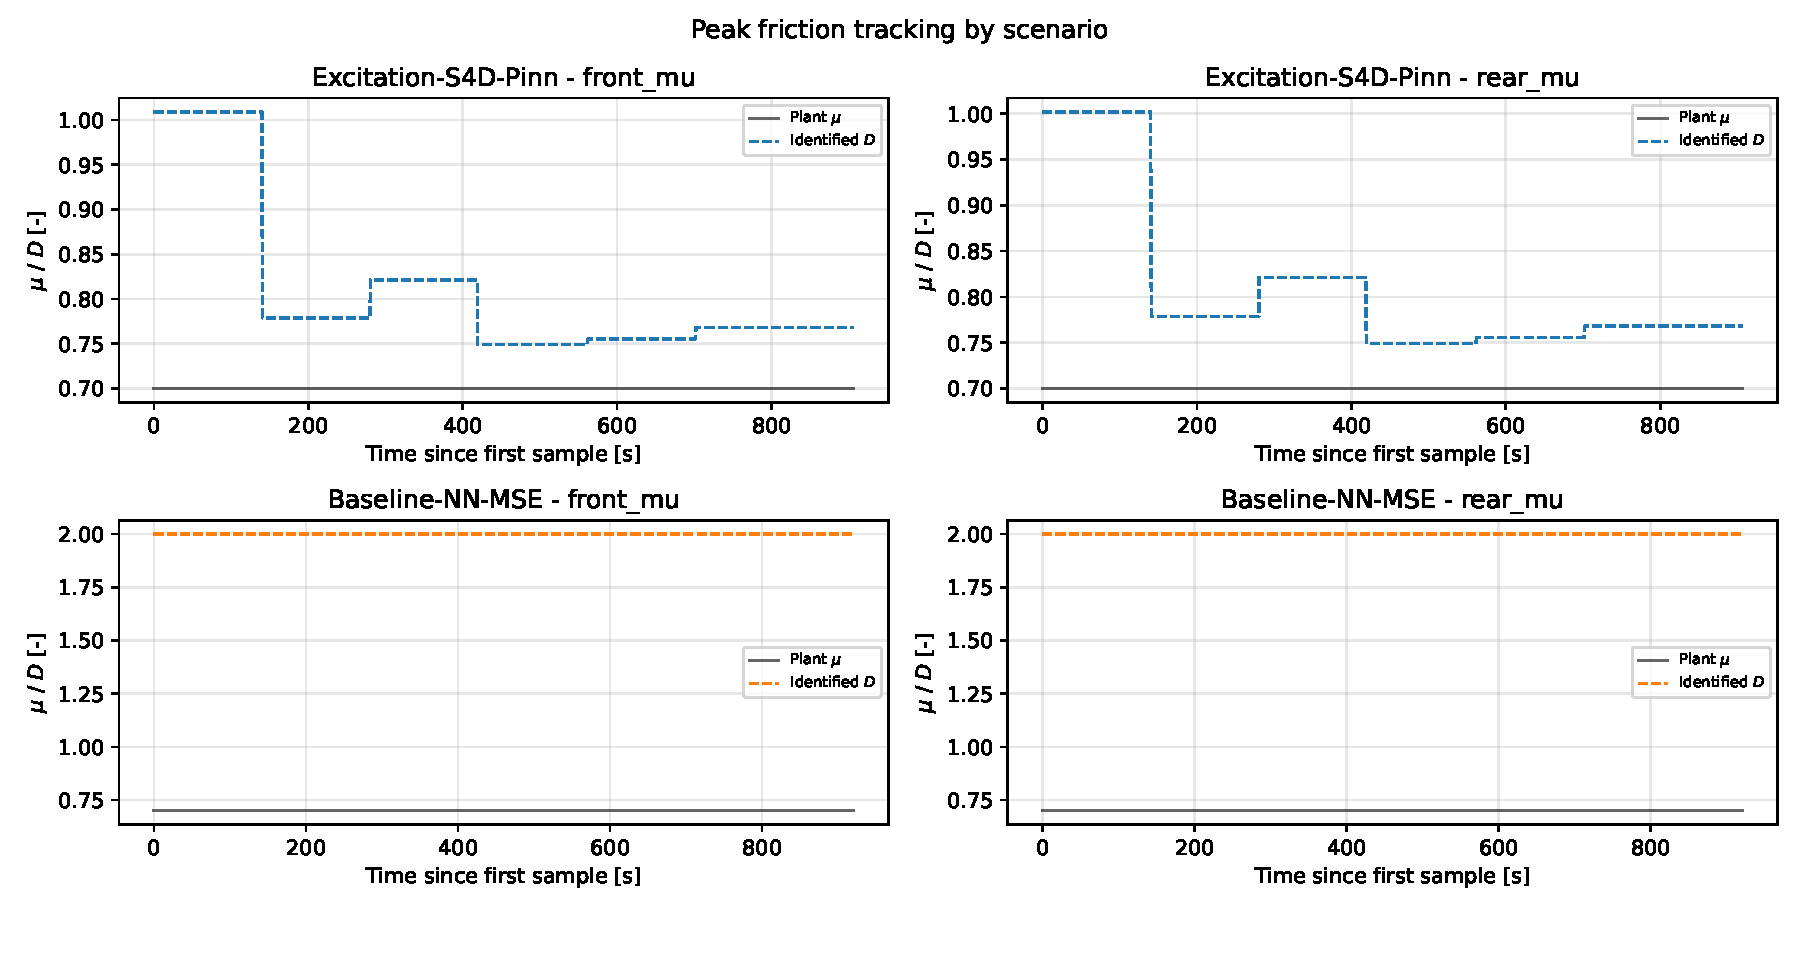
\includegraphics[trim=0 25 431 26, clip, width=\textwidth]{Figures/mu_timeseries_by_scenario_constant_mu.pdf}
\caption{Peak friction over the run on the static surface, front axle, one row
per configuration: the plant's effective $\mu$ (black) against the identified
peak factor $D$ published at each accepted identification. The rear axle is
identical and is omitted, since $D$ is pinned to the same value on both axles
(Section~\ref{subsec:frictionfloor}). Every departure from the black line is
estimator error: \oursarm{} publishes the $\mu=\num{1.05}$ prior while the gate
is closed, steps down onto the plant within \SI{11}{\percent} at the first
release, and holds. \basearm{} sits on the $D\le\num{2.0}$ box constraint
throughout.}
\label{fig:mutimeseries}
\end{figure}

\begin{figure}[htbp]
\centering
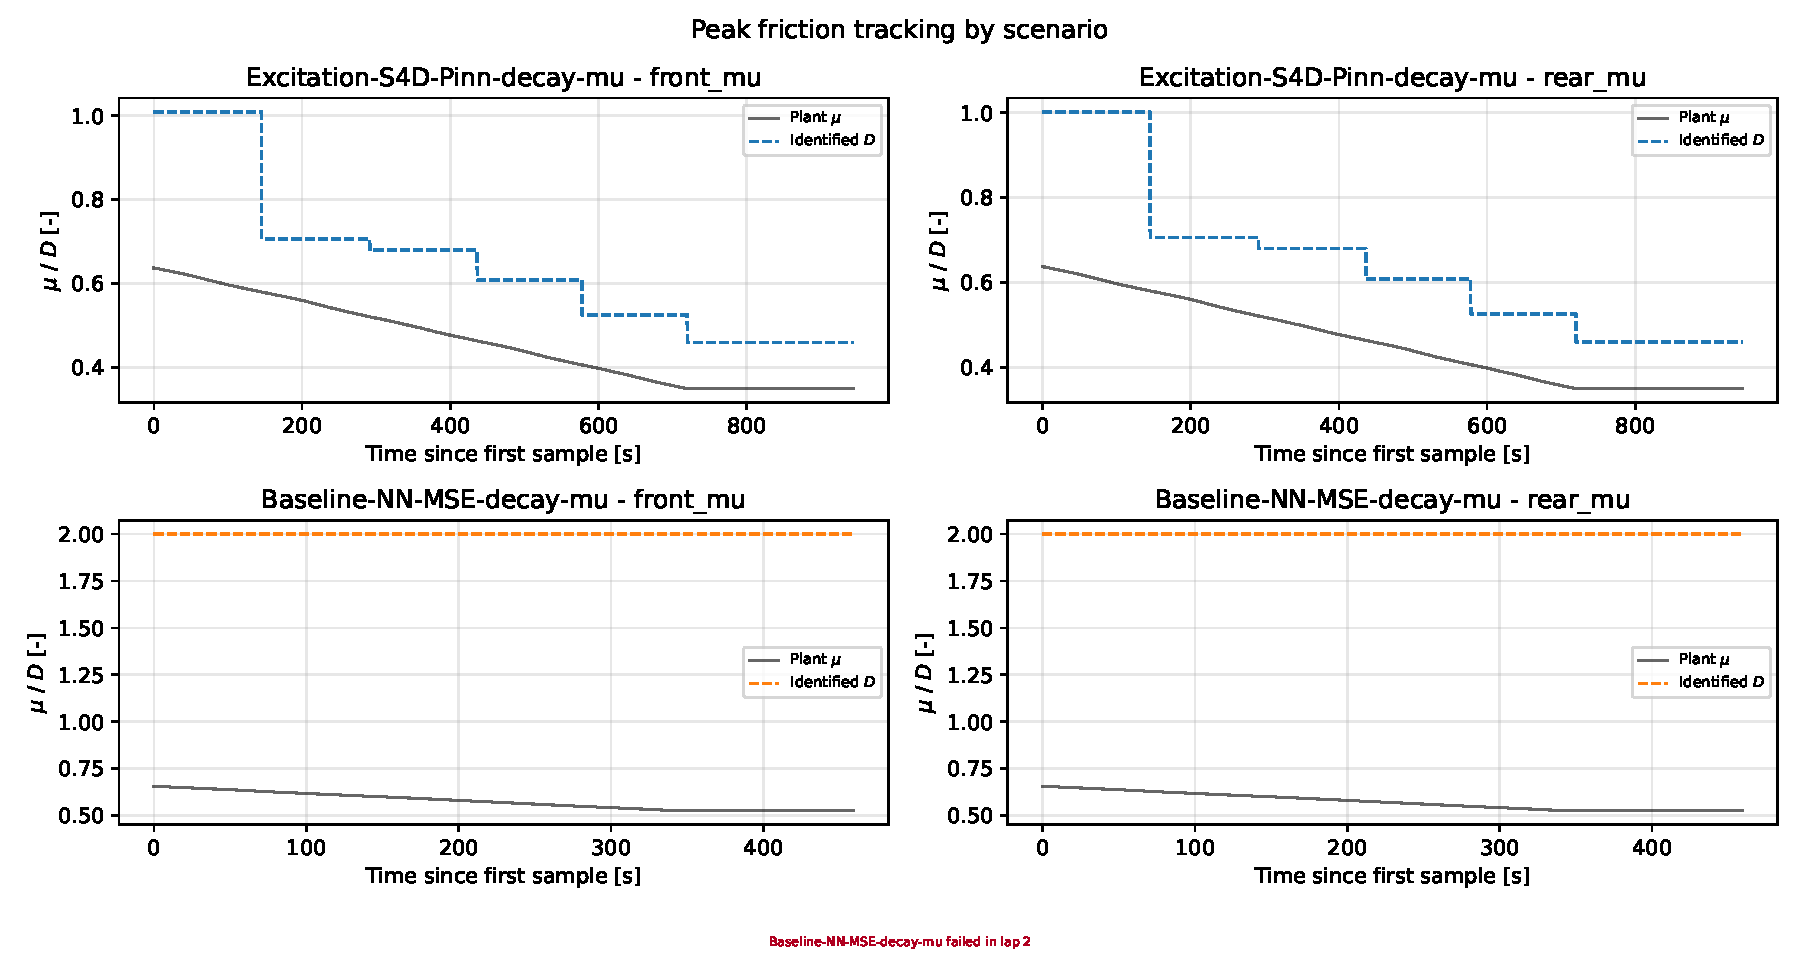
\includegraphics[trim=0 25 431 26, clip, width=\textwidth]{Figures/mu_timeseries_by_scenario_decay_mu.pdf}
\caption{Peak friction over the run on the decaying surface, drawn exactly as
Figure~\ref{fig:mutimeseries}. The five accepted \oursarm{} cycles walk the
published $D$ down at \SI{7}{\percent} of the plant's own rate, offset by one
cycle of transport lag and by the same estimator bias the static surface shows.
\basearm{} again sits on the $D\le\num{2.0}$ box constraint, and its trace ends
where the car left the track.}
\label{fig:mutimeseriesdecay}
\end{figure}

\subsection{Axle lateral force and one-step state prediction}
\label{subsec:resultsforce}

The identified curve is scored at the measured $(\alpha,F_{z})$ against the
plant's own lateral force, summed per axle (Table~\ref{tab:comparison}). On the
static surface \oursarm{} leads on both axles by an order of magnitude in RMSE
and in the error tails; the baseline's negative $R^{2}$ means its curve predicts
the plant's axle force worse than the mean of that force does. This is the
linear-range result seen as force: at $P_{99}(|\alpha|)=\SI{2.7}{\degree}$ the
metric is dominated by cornering stiffness, so the models separate almost
entirely on slope. Because $D$ multiplies that slope in Eq.~\eqref{eq:stiffness},
\basearm{}'s railed $D$ is the direct cause of its force error. Pinning $D$
alone does not produce these numbers: with $\beta=1$ the same arm degrades
monotonically with iteration count (Section~\ref{subsec:ablations}), which is
why the relaxed update of Eq.~\eqref{eq:relax} belongs in the method rather than a
configuration file.

On the decaying surface \oursarm{}'s force error grows by about a fifth,
\SI{32.9}{\newton} front against \SI{27.2}{\newton}, which is the transport lag
of Section~\ref{subsec:resultsmu} converted into force, and $R^{2}$ stays at
\num{0.984} and \num{0.977}. \basearm{}'s force error is \emph{lower} there than
on the static surface, \SI{171.4}{\newton} against \SI{329.6}{\newton}, and its
$R^{2}$ turns positive. That is not a success: its run is scored over \num{2597}
samples against \num{10744}, it ends before the surface reaches its floor, and
its worst-case error is the largest in the table at \SI{2507}{\newton}. A model
with five coefficients on a box edge produced a better-looking aggregate over a
shorter and slower run, which is the diagnostic problem
Section~\ref{subsec:identifiability} describes.

Level~1 of the validation protocol is reported against a persistence baseline
(next state equals last measured state) written by the same benchmark node.
\oursarm{} leads on both signals on both surfaces, by an order of magnitude on
lateral velocity on the static surface ($R^{2}$ \num{0.998} against
\num{0.709}) and by a factor of two on yaw rate ($R^{2}$ \num{0.892} against
\num{0.527}). Neither model beats persistence at the \SI{0.035}{\second} model
step for either configuration or signal, because a one-step metric on a smooth
trajectory rewards not moving. One-step accuracy is therefore weak evidence for
either tire model, and the gap is read only as confirming the direction the
axle-force and closed-loop comparisons establish.

\subsection{Closed-loop tracking}
\label{subsec:resultsclosedloop}

Figures~\ref{fig:overlay} and~\ref{fig:overlaydecay} cover the whole of each
run.

On the static surface both arms finish three timed laps with zero emergency
halts and the same finite-state sequence, with the handover at
$t=\SI{79.1}{\second}$ for \oursarm{} and $t=\SI{64.0}{\second}$ for
\basearm{}. Under MPC, where the identified model enters the loop, \oursarm{}
tracks at \SI{0.151}{\meter} RMS lateral error against \SI{0.224}{\meter}, a
\SI{32}{\percent} reduction, with maximum \SI{0.683}{\meter} against
\SI{0.776}{\meter}. ITAE is $\int t|e_{y}|\,\mathrm{d}t$, neither scale-free
nor comparable across runs of different length, so the duration-normalised
forms $\mathrm{IAE}/T=\num{0.104}$ against \num{0.157} and
$\mathrm{ITAE}/(T^{2}/2)=\num{0.095}$ against \num{0.166} are reported beside
it; all three order the runs alike. The split by controller confirms that the
whole difference sits in the MPC phase: the pure-pursuit phases, which do not
use the identified model, give \num{110} and \num{107}, within
\SI{3}{\percent} of each other. The QP cost is unchanged, both arms staying two
orders of magnitude below the \SI{50}{\milli\second} control period; the
identified coefficients change the model the QP carries, not its size.

On the decaying surface the two arms separate at $t\approx\SI{246}{\second}$,
in lap~2. \basearm{}'s lateral error steps from under \SI{1}{\meter} to
\SI{38.4}{\meter} inside a few seconds, its speed goes through zero to
$-16.9\,\si{\meter\per\second}$, and the run ends on a collision whose horizontal
impulse of \SI{415.9}{\newton\second} is twice the \SI{200}{\newton\second}
abort threshold. The plant's effective $\mu$ at that moment is \num{0.525},
worth \SI{0.53}{\g}, against a reference that is still asking for
\SI{0.51}{\g} at its peak and a model that is still reporting a
\SI{2.00}{\g} ceiling. The failure is not a tracking degradation that grew
until it mattered; the tracking error is flat and small right up to the
departure, which is what a grip limit being crossed looks like from inside the
controller.

\oursarm{} completes its three laps on the same surface and its tracking error
does not degrade as the grip halves: binned in \SI{100}{\second} windows after
the handover it reads \num{0.153}, \num{0.138}, \num{0.155}, \num{0.094},
\num{0.152} and \SI{0.092}{\meter} RMS, with no trend, against \num{0.123} to
\SI{0.179}{\meter} over the corresponding windows of the static-surface run.
What moves instead is the speed. The identified grip ceiling falls with the published $D$, the
controller re-clamps the reference speed profile against it, and the peak
lateral demand of the clamped reference drops from \SI{4.98}{\meter\per\second\squared}
(\SI{0.51}{\g}) at the start of the run to \SI{2.92}{\meter\per\second\squared}
(\SI{0.30}{\g}) at the end. The three lap times lengthen accordingly, to
\num{189.8}, \num{160.9} and \SI{169.2}{\second} against \num{175.2},
\num{145.4} and \SI{142.8}{\second} on the static surface, an \SI{18}{\percent}
loss on the last lap. That trade is the argument for identifying on
track: the vehicle pays lap time it has to pay, and the identification is what
tells it how much. \basearm{} never makes the trade, because a peak factor
pinned to a box constraint cannot tell the controller that anything has
changed. Lap times themselves are not read as a vehicle-performance result
across arms, for the clock reason of Section~\ref{subsec:setup}; the comparison
that carries this paragraph is within the \oursarm{} column, where the same
configuration meets two surfaces.

\begin{figure}[htbp]
\centering
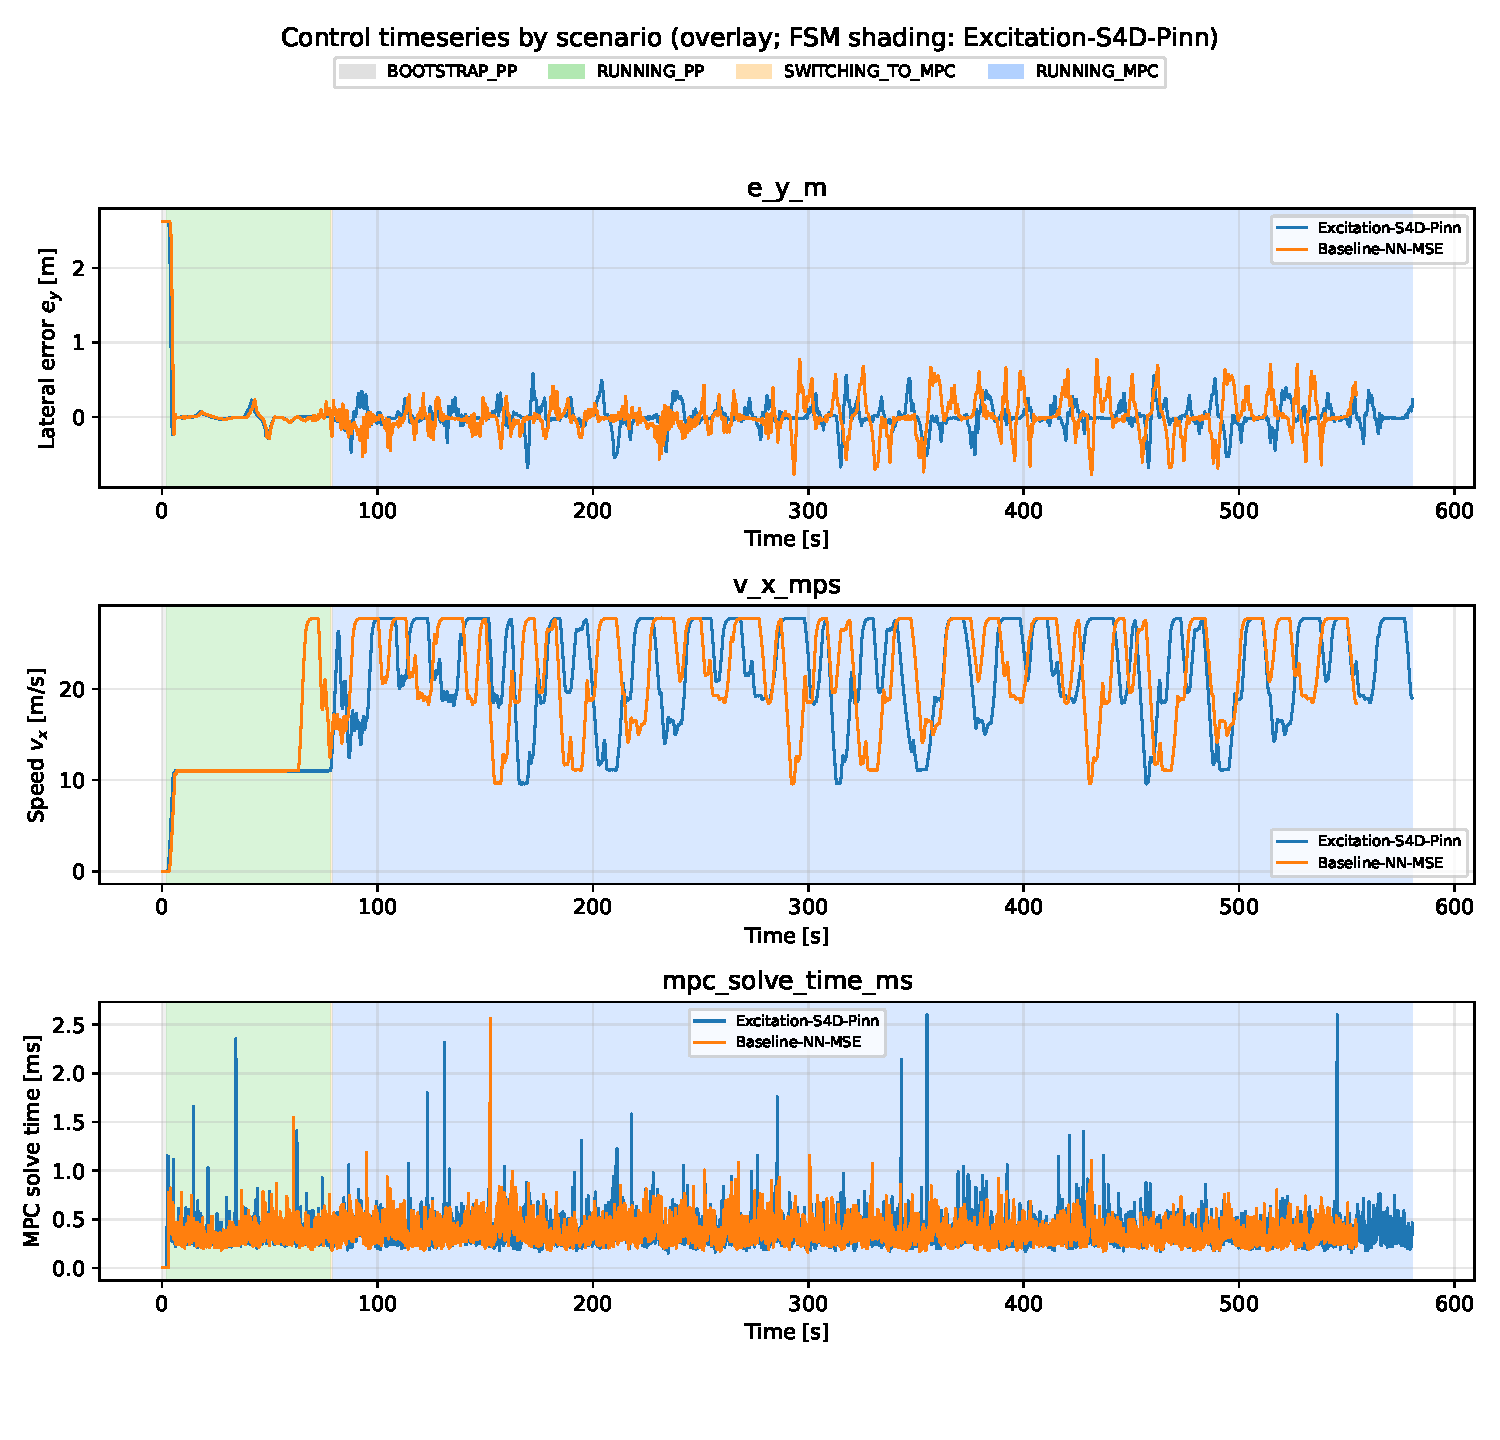
\includegraphics[width=\textwidth]{Figures/control_timeseries_overlay_by_scenario_constant_mu.pdf}
\caption{Lateral error, longitudinal speed and MPC solve time over the whole of
the static-surface run, both configurations overlaid, shaded by the active
controller state of the \oursarm{} arm. Both arms run to three laps and the
traces stay superimposed. Solve time stays two orders of magnitude below the
\SI{50}{\milli\second} control period.}
\label{fig:overlay}
\end{figure}

\begin{figure}[htbp]
\centering
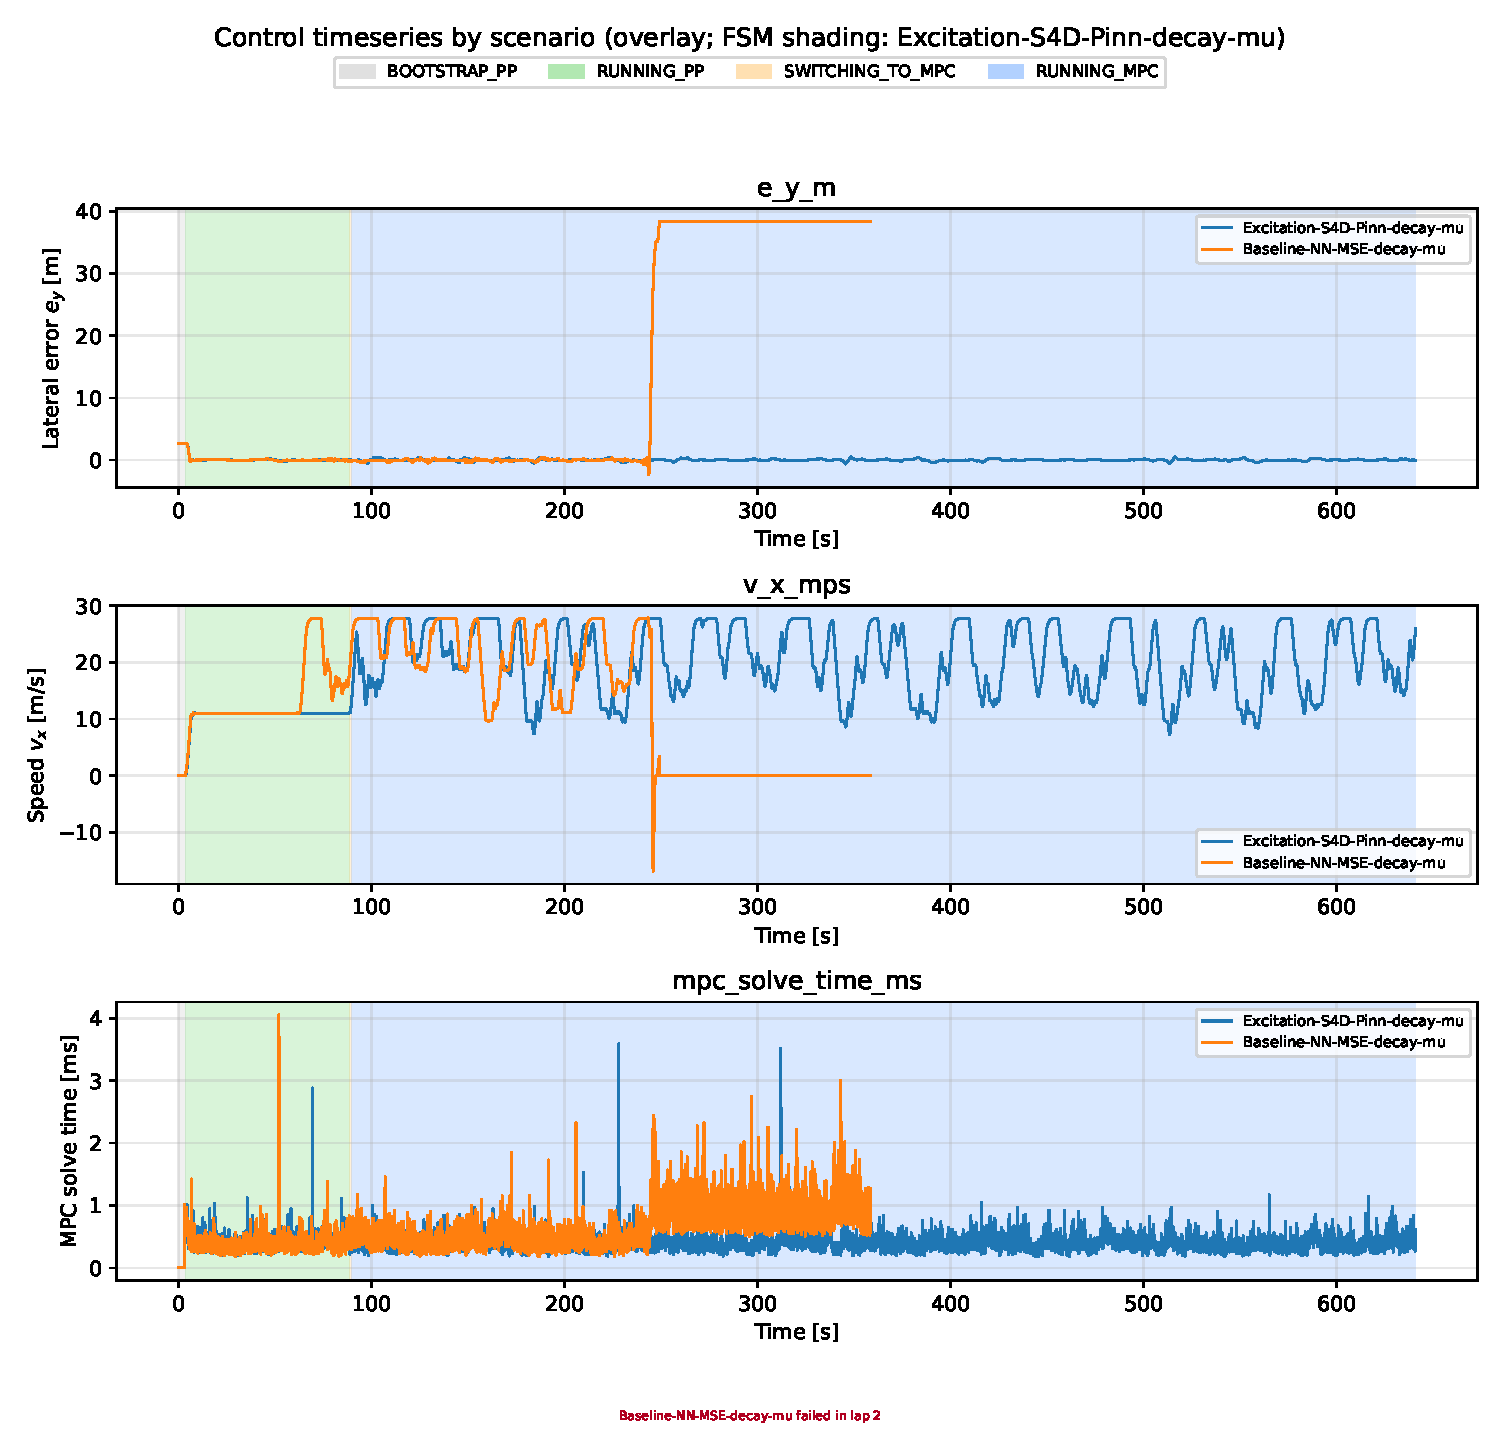
\includegraphics[width=\textwidth]{Figures/control_timeseries_overlay_by_scenario_decay_mu.pdf}
\caption{The same three signals over the decaying-surface run, drawn exactly as
Figure~\ref{fig:overlay}. \basearm{} departs the track at
$t\approx\SI{246}{\second}$ ($e_{y}$ to \SI{38.4}{\meter}, speed through zero)
while \oursarm{} runs to \SI{640.9}{\second}. \oursarm{}'s speed trace loses its
peaks over the second half of the run: the controller re-clamps the reference
against a grip ceiling that is falling because the identifier says it is.}
\label{fig:overlaydecay}
\end{figure}

\subsection{What carries the result}
\label{subsec:ablations}

The two arms differ in nine settings at once, so the comparison above
establishes an ordering and attributes nothing. Appendix~\ref{sec:ablations}
attributes it by offline replay of the identification stage on the five
\SI{30}{\second} buffers each arm collected during its own run, scored with the
quantity the closed-loop tire-force benchmark reports. Four settings carry the
result. Refusing to fit an unmeasured $D$ removes most of the error, cutting the
mean $|D-\mu|$ from \num{0.585} to \num{0.084} on replayed buffers of a
$\mu=\num{1.05}$ run. Damping the loop carries the rest: axle force RMSE is
\num{70.4} and \SI{62.3}{\newton} at the inherited $\beta=\num{1.00}$,
\num{92.5} and \SI{71.8}{\newton} at $\beta=\num{0}$, which is no
identification at all, and \num{28.0} and \SI{19.4}{\newton} at the
$\beta=\num{0.20}$ that ships. Normalising the physics-informed objective is
necessary but not sufficient alone, and the S4D residual is worth
\SI{21}{\percent} on the force metric at matched settings. Two settings buy
nothing measurable: the residual \emph{objective}, indistinguishable from a
plain one-step MSE once the normalisation and the damping are both in place,
and the fast-$\mu$ derate, which sat at the upper end of its
$[\num{0.4},\num{1.2}]$ clamp over the last cycles of the decaying run, so the
reference re-clamp of Section~\ref{subsec:resultsclosedloop} is carried by the
published $D$ and not by the derate.

\subsection{Identification cost}
\label{subsec:runtime}

One S4D identification, six co-identification iterations on a \SI{30}{\second}
lap, takes \SI{20.9}{\second} end to end, inside the \SI{30}{\second}
re-identification period. The reduction from the \SI{181.4}{\second} it
originally took is exact: no epoch count, iteration count, early-stopping rule
or loss weight changed, and the identified coefficients agree to four decimal
places. That margin is what makes the decaying-surface result possible at all,
and it is also what bounds it: one cycle of lag on a surface moving at
Eq.~\eqref{eq:decay}'s rate costs the \SIrange{10.9}{17.4}{\percent} offset of
Section~\ref{subsec:resultsmu}, and a surface moving ten times faster would cost
ten times that. The per-phase breakdown is in the supplementary material.

% === VII. INTEGRATION WITH THE CONTROLLER ====================================
\section{Integration with the Controller}
\label{sec:integration}

The identified model leaves the pipeline through one interface. A nonlinear MPC
path-tracking controller (acados~\cite{acados2022}, partial-condensing
HPIPM~\cite{hpipm2020}, horizon $N=20$, run at \SI{20}{\hertz})
carries the same single-track model as the identifier and consumes $\phip$
directly through Eq.~\eqref{eq:mf}, pushed over a ROS~2 service at the end of each
identification cycle. We claim no contribution to the controller design; it
appears here as the consumer that defines what an admissible identification is.

\subsection{Admissibility gates}
\label{subsec:gates}

A coefficient set can lie strictly inside every box constraint and still be
unusable. We observed two ways, each requiring a gate on a \emph{derived}
quantity, not on a coefficient:

\begin{enumerate}
\item \textbf{Grip ceiling versus trajectory demand.} The controller computes
$\max_{k}(v_{x,k}^{2}|\kappa_{k}|)$ over the speed-clamped reference, rejects
any identification whose $a_{y}^{\max}$ from Eq.~\eqref{eq:gripceiling} falls below
it, and otherwise re-clamps the reference speed profile against that ceiling,
which is the path by which a falling peak factor slows the vehicle in
Section~\ref{subsec:resultsclosedloop}. On the earlier trajectory the degenerate
fit reported a \SI{0.40}{\g} ceiling against a \SI{1.22}{\g} demand and produced
\SI{41.89}{\meter} of cross-track error at \SI{27}{\meter\per\second}, against
\SI{0.03}{\meter} for a physically plausible set ($D=\num{1.5}$) on the same
trajectory, at the same speed and through the same controller; the same
identified set gives \SI{0.16}{\meter} at \SI{11.1}{\meter\per\second}, the
$v^{2}$ scaling the Introduction describes. These figures come from an offline
closed-loop harness and not from a controlled pair of simulator runs, and are
quoted as the observation that motivated the gate, not as a result. The gate is
one-sided by construction and catches only a ceiling that is too low, so
\basearm{}'s \SI{2.00}{\g} (Section~\ref{subsec:resultstire}) passes it on both
surfaces, which is why the decaying-surface departure is visible in the
controller and not at this interface.
\item \textbf{Understeer sign and critical speed.} A set with
$l_{f}C_{f}>l_{r}C_{r}$ whose $v_{\mathrm{crit}}$ falls inside the controller's
speed range makes the prediction model open-loop unstable, and the resulting
$\rho(A_{d})>1$ is raised to $\rho^{N}$ in the condensed QP. An observed set
gave $C_{f}=\SI{37031}{\newton\per\radian}$ against
$C_{r}=\SI{11691}{\newton\per\radian}$, i.e.\
$v_{\mathrm{crit}}=\SI{14.5}{\meter\per\second}$ at the measured geometry and
mass of Table~\ref{tab:vehicle}, inside the controller's speed range on every
trajectory in this paper.
\end{enumerate}

A third observation is a controller-implementation detail rather than a gate on
the identification: an admissible set can still be stiff relative to the control
period, so the prediction model sizes its RK4 sub-step from its own fastest
lateral mode, restoring $\rho\approx1.000$ across the speed range, at a median
QP setup-and-solve cost of \SI{0.36}{\milli\second} against the
\SI{50}{\milli\second} control period.


An identification that passes the gates is a model the controller can be held
responsible for; one that fails is reported as unidentified rather than
deployed. Two further controller-side changes were required before any
identified model could be evaluated at full-scale speeds: reference speeds are
clamped at ingest, and the solved state is rolled forward by the measured
transport delay before each solve. Both are recorded for completeness and are
not identification results.

% === VIII. DISCUSSION AND LIMITATIONS ========================================
\section{Discussion and Limitations}
\label{sec:disc}

\subsection{What generalises, and what does not}

The reachable-friction bound~Eq.~\eqref{eq:mureach} is kinematic: it involves no
tire parameter, no simulator-specific quantity and no property of the residual
model, so it applies to any implementation of the virtual-steady-state-data
strategy of~\cite{ontrack2025}, in simulation or on hardware. Its practical
content is a design rule: the rollout must be configured to demand at least the
friction one intends to identify, and where it cannot, $D$ should be reported
as unidentified and not fitted. The diagnostic signature, coefficients
resting exactly on box constraints, is likewise generic and should be checked
and logged by any bounded tire-fitting routine, being otherwise
indistinguishable in the output from a successful fit. The two structural
properties of Section~\ref{subsec:contraction} generalise on the same grounds:
the $BCD$ degeneracy follows from the quasi-steady force recovery
Eq.~\eqref{eq:ssforces}, and the absence of contraction from stage~4 alone. What
does not generalise is the value \num{0.20}, a property of this vehicle's
extrapolation error; what does is that $\beta=1$ is not defensible and
$\beta=0$ worse still. The insufficiency of per-coefficient box constraints is
also platform-independent, and the decaying surface adds a third instance to
the two we had: a stiffness that looks right while being the product of a
railed $B$ and a railed $D$, carried by a controller until the surface fell
below the reference's demand.

Three results are properties of this plant and must not be read as statements
about tires: the numerical tire values, since the plant is a PhysX
wheeled-vehicle model; the gap between configured wheel friction and realised
peak axle friction (\num{1.0} against \num{0.70}), which we report because an
identifier tuned to converge on the configuration file's number will converge
on the wrong one; and the \num{0.76} achieved/commanded steering ratio, where
the lesson (identify against the achieved actuator state) is general but the
magnitude is not. Sagmeister
\emph{et al.}~\cite{simfidelity2026} show sensitivity to model fidelity is
largest near the acceleration limits, where this study operates, and
R-CARLA~\cite{rcarla2025} exists because CARLA's native dynamics are a known
weak point for racing-grade work, so hardware replication is necessary before
any claim about identification accuracy on a real vehicle.

\subsection{Limitations}
\label{subsec:limits}

\begin{enumerate}
\item \textbf{One run per configuration and surface, so no metric in
Table~\ref{tab:comparison} carries an uncertainty.} The \SI{0.151}{\meter}
against \SI{0.224}{\meter} RMS tracking difference in particular has no
confidence interval and no evidence that it exceeds run-to-run variation, which
is not measured here; the order-of-magnitude force and friction margins are
large enough that such variation is unlikely to reverse them, but that is an
argument, not a measurement. The decaying-surface departure is a single event
and identifies a failure \emph{mechanism}, a grip ceiling pinned to a box
constraint while the plant falls below the reference's demand, not a failure
rate.
\item \textbf{One decay law, at one rate, on one vehicle and trajectory.} The
schedule is linear at \SI{0.1}{\percent} of nominal per second with a floor at
half, a factor \num{20} slower than the \SI{2}{\percent} per second
of~\cite{llampc2025}, for the reason Section~\ref{subsubsec:surface} gives: a
faster decay outruns the \SI{30}{\second} buffer this class of identifier is
built on, so the experiment would measure the sampling period rather than the
estimator. The runs therefore establish that the pipeline tracks a friction
change slow relative to its own cycle, with the scaling of
Section~\ref{subsec:runtime}. Step changes, which the scenario file also
carries, are not run, and the lag the decay exposes would appear on a step as
an overshoot of the whole cycle.
\item \textbf{The two surfaces were run on different controller builds.} The
decaying-surface pair carries a grip rate limiter, a binding-axle derate and the
fast-$\mu$ hook of Table~\ref{tab:scenarios}, none of which are in the
static-surface pair. Within each pair the two arms are identical apart from
Table~\ref{tab:scenarios}, so each comparison is clean; across pairs, only the
\oursarm{} lap-time and tracking-error trend is read.
\item \textbf{The friction estimator's excitation sweep is synthetic}
(Appendix~\ref{subsec:mu}), so the excitation dependence of its
\SI{11}{\percent} bias is not mapped against the simulator's per-wheel forces.
The published peak factor is exactly this estimate, so the bias passes through
undamped, and on the decaying surface it arrives with one cycle of lag on top
of it. Relatedly, the rear axle is not identified on this trajectory and the
front-axle $\mu$ is applied to both (Section~\ref{subsec:frictionfloor}); the
quasi-steady argument making $\mu_{f}=\mu_{r}$ holds on a homogeneous surface
and would not survive a split-$\mu$ one, which this sensor set cannot detect in
the first place.
\item \textbf{The two configurations differ in nine settings at once}
(Table~\ref{tab:scenarios}), so Section~\ref{subsec:summary} attributes nothing
to any one of them. Section~\ref{subsec:ablations} does attribute four, but by
offline replay on recorded buffers, so its ordering is not a closed-loop
ordering, and the integrator, the sweep bound and the regularisation are not
separated at all. The S4D figure there (\SI{21}{\percent} on force RMSE at
matched settings) has the same status: a measured ablation, not a reproduction
of the closed-loop S4 improvement of~\cite{visionsysid2026}. The
excitation-aware rollout, this paper's central contribution, is active in
\emph{both} arms, so the closed-loop comparison is not evidence for the
identifiability correction; the evidence for that is the sweep of
Section~\ref{subsec:sweep}.
\item \textbf{The physics-informed objective buys nothing measurable here.}
Once its units are reconciled with the data term and the loop is damped, it is
indistinguishable from a plain one-step MSE on this manoeuvre. It is retained
because it is the paper's stated formulation and costs nothing, not because it
is shown to help.
\item \textbf{Longitudinal dynamics are out of scope.} As in the baseline, only
lateral dynamics are identified. Combined slip and load transfer are neglected,
and the simulator's longitudinal wheel force channel is drivetrain torque rather
than a contact-patch force, so it is unusable as ground truth for a longitudinal
extension without further work.
\end{enumerate}

% === IX. CONCLUSION ==========================================================
\section{Conclusion and Future Work}
\label{sec:conclusion}

This paper studied the identifiability of a learning-based on-track Pacejka
identification pipeline~\cite{ontrack2025} at full vehicle scale, using a CARLA
simulation architecture that exposes the plant's own per-wheel forces as ground
truth. Transplanted unchanged from a 1:10 platform, the pipeline fails in a
specific, diagnosable and correctable way: a loss of excitation created by its
own virtual-data step, which no change of solver, bounds or tuning removes, and
whose reachable friction depends on the rollout configuration and not the tire.
Two further properties of the loop follow from the same analysis. Stage~3
reconstructs its forces from the rollout's own quasi-steady yaw balance, so its
residual depends on $B$, $C$ and $D$ only through their product and the peak
factor is not recoverable from the rollout at any excitation; it must be
measured on the recorded trace and held. And each fit is handed the trajectory
its own previous answer generated, so stage~4 is a positive feedback path
rather than a contraction and is reformulated as a relaxed fixed-point
iteration at $\beta=\num{0.20}$. The correction ships with an extrapolation
bound on the steering sweep, a frozen regularisation target, identification
against the achieved road-wheel angle, measured mass and geometry, and a
dynamics residual normalised to the units of the data term, and it produces
accepted identifications with no railed coefficient and the correct understeer
sign.

A second surface settles what a single one cannot. With the plant's friction
driven down under the moving vehicle on the linear-decay protocol
of~\cite{llampc2025} until half the grip is gone, the corrected pipeline
recovers the decay rate to \SI{7}{\percent} and the level to
\SIrange{10.9}{17.4}{\percent} once one cycle of transport lag is accounted
for; the falling peak factor re-clamps the reference from \SI{0.51}{\g} of peak
lateral demand to \SI{0.30}{\g}, buying three completed laps at unchanged
tracking error for \SI{18}{\percent} of lap time. The inherited configuration
leaves the track in lap~2, holding a \SI{2.00}{\g} grip ceiling against a plant
offering \SI{0.53}{\g}. Both outcomes have one cause: a peak factor resting on
a box constraint cannot report that anything changed, so the identifier's
failure stays invisible until the controller acts on it.

Two qualifications stand on those numbers: the peak factor is identified by the
brush estimator on the recorded trace, not by the Pacejka fit, which cannot
identify it (Section~\ref{subsec:bcd}); and each configuration is a single run
per surface, so the closed-loop margins are observations rather than estimates
with a confidence interval. We further argue that per-coefficient box
constraints are not a sufficient admissibility criterion for handing a model to
a model-based controller, and place gates on derived physical quantities at
that interface instead.

\subsection{Future work}

\begin{enumerate}
\item \textbf{Shorten the cycle, or step the friction.} The decay runs expose
one cycle of transport lag as the dominant error on a moving surface, worth
\SIrange{10.9}{17.4}{\percent} at the rate used here and proportionally more at
a faster one. Two experiments follow directly, both scenario-file rows: the step
schedules, on which the same lag appears as a bounded overshoot rather than a
standing offset, and a shorter re-identification period, which the
\SI{20.9}{\second} cycle cost of Section~\ref{subsec:runtime} leaves room for.
\item \textbf{Run the ablations of Section~\ref{subsec:ablations} in the loop.}
The relaxation sweep, the $D$-pinning comparison and the S4D and objective
ablations are offline replays, enough to attribute the result but not to confirm
the ordering survives closed-loop coupling. Each is a scenario-file row.
\item \textbf{Excite the peak, and design for it.} The lap reaches
$P_{99}(|\alpha|)=\SI{2.7}{\degree}$ against a plant whose curve peaks at
\SI{8.0}{\degree}, which is where the brush estimator's \SI{11}{\percent} bias
comes from. Eq.~\eqref{eq:mureach} inverts into a requirement on the
manoeuvre, so a controller that inserts bounded slalom or ramp-steer excitation
when the identifier reports insufficient slip-angle coverage would move the
pipeline toward active, safety-bounded experiment
design~\cite{goodwin1977design}.
\item \textbf{Hardware replication.} The decisive test of every claim in
Section~\ref{sec:disc} is a physical Formula Student vehicle. The identification
code is unchanged between simulation and hardware; what changes is the
availability of ground truth, which is what makes the simulation study a
necessary precursor rather than a substitute.
\end{enumerate}

\bibliographystyle{sn-nature}
\bibliography{references}

%%=============================================================================
\begin{appendices}

% === APPENDIX ================================================================
\section{Assumptions and Reproducibility Notes}
\label{subsec:assumptions}

The following are assumptions or design choices rather than measured facts,
listed so a reader can judge how far each result depends on them.

\emph{A1. Yaw inertia.} $I_{z}=\SI{51.1}{\kilo\gram\meter\squared}$ is carried
in the model file and is \emph{not} measured. It enters Eq.~\eqref{eq:omdot}
directly, so it scales the yaw-rate residual the network is trained on. It can
be discharged by applying a known yaw moment and fitting $I_{z}$ from the
measured $\dot\omega$, or by reading the actor's inertia tensor.

\emph{A2. Centre-of-gravity split.} $l_{f}=\SI{0.738142}{\meter}$,
$l_{r}=\SI{0.795362}{\meter}$ are taken from the controller configuration. The
measured static load split (51.2/48.8) implies a marginally different split than
the geometry does (51.9/48.1), a \SI{1.4}{\percent} disagreement, below the
level at which any conclusion here would change.

\emph{A3--A4. CG height and steering sign.} $h_{\mathrm{cg}}=\SI{0.3}{\meter}$
is carried but not measured. The single-track identification model neglects
load transfer, following the baseline, and its normal loads are static; the
only consumer of $h_{\mathrm{cg}}$ is the longitudinal transfer term of the
friction warm start (Section~\ref{subsec:friction}), where it moves the axle
loads by up to \SI{14}{\percent} at the \SI{0.35}{\g} the fit admits. \texttt{feedback/\allowbreak
steering\_angle} is published in degrees and treated as the front road-wheel
angle, positive left, verified against the front-left wheel joint state to
within \SI{0.5}{\percent}; left and right road wheels are not distinguished.

\emph{A5. Steady-state force recovery.} Eq.~\eqref{eq:ssforces} is not a
force measurement; being fully determined by $v_{x}\omega$ it misattributes
transients, and it is applied only to the \emph{synthetic}, quasi-steady
rollout. Its adequacy was checked on measured data against the simulator's own
axle force (correlation \num{0.993}, slope \num{0.94}).

\emph{A6. The residual network is not the plant.} The corrected model is queried
by the rollout at inputs the network has only partially seen. The extrapolation
bound of Section~\ref{subsec:iterative} limits but does not eliminate this: the
sweep still reaches $1.5\times$ the observed 99th percentile of $|\delta|$, a
choice that is empirical rather than derived.

\emph{A7. Simulator determinism and timing.} CARLA runs in synchronous mode with
a \SI{0.033}{\second} physics step; sim time advances faster than wall time, at
a ratio set by the host load and therefore not identical across runs
(between \num{1.28} and \num{1.66} on the four runs of
Section~\ref{sec:results}). All
identification and force-validation data is stamped from the simulation clock,
while the controller node stamps its own metrics on the wall clock; the two are
never mixed inside one metric (Section~\ref{subsec:setup}).

\emph{A8. Software configuration of record.} ROS~2 Humble, Python 3.10, PyTorch
with CUDA on an RTX~2080-class GPU; the bridge is a separate overlay; CARLA
server 0.9.16 / Unreal Engine 4.26; acados 0.5.5 with partial-condensing HPIPM.
The identifier's acquisition timer runs at \SI{50}{\hertz} (the controller runs
at \SI{20}{\hertz}, a \SI{50}{\milli\second} period) with a \SI{30}{\second}
buffer, six co-identification
iterations, 200 training epochs, full-batch Adam at $5\times10^{-4}$, and
$T_{s}=\SI{0.035}{\second}$. \texttt{nn\_train} seeds PyTorch and NumPy at
\num{42}; \texttt{pacejka\_solver.seed} is \texttt{null} in both shipped
parameter sets, so the reported identifications are reproducible in distribution
but not bit for bit, while the sweep of Table~\ref{tab:sweep} is seeded
explicitly and is bit-reproducible.

\emph{A9. Reference trajectory.} Figure~\ref{fig:raceline} shows the raceline
all four runs follow and the lateral demand it places on the plant.

% Landscape diagram: upright it scales to two thirds and its labels stop
% being legible, so it is rotated, as the template asks for oversize content.
\begin{sidewaysfigure}
\centering
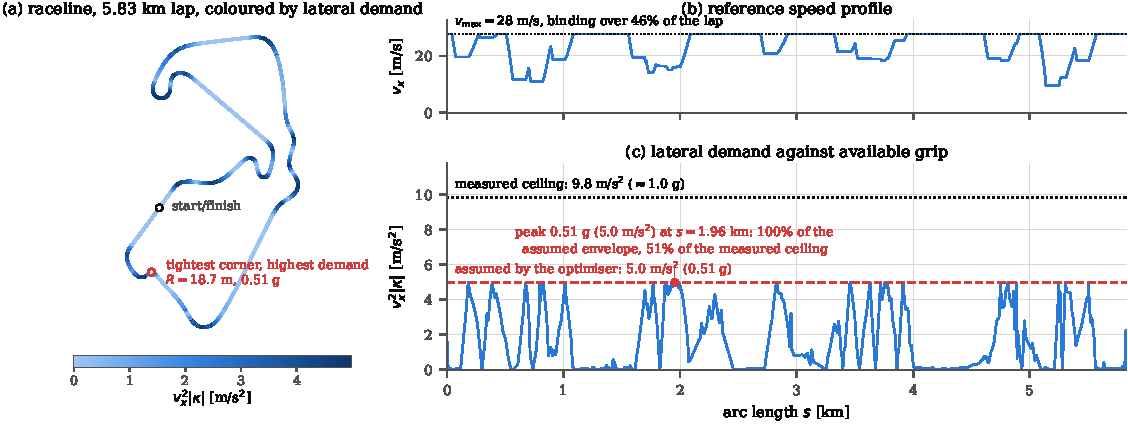
\includegraphics[width=\textheight]{Figures/raceline.pdf}
\caption{The optimised raceline used for all four
runs~\cite{tumracetraj,heilmeier2020}. (a) Track layout, coloured by lateral
demand, with the marked corner ($R=\SI{18.7}{\meter}$) the tightest on the lap.
(b) Reference speed profile. (c) Lateral demand $v_{x}^{2}|\kappa|$ along the
lap against the flat \SI{5.0}{\meter\per\second\squared} envelope handed to the
optimiser (dashed) and the grip the vehicle has on the static surface (dotted,
$\approx\SI{0.70}{\g}$, measured). No segment exceeds the plant's grip there;
on the decaying surface the dotted line falls through the solid one.}
\label{fig:raceline}
\end{sidewaysfigure}


\section{Peak-Friction Warm Start on a Synthetic Plant}
\label{subsec:mu}

The friction warm start is evaluated on a synthetic single-track plant with
brush tires, because only a synthetic plant supplies a $\mu$ known exactly and
an excitation level that can be swept independently of it: a swept-sine steering
input for \SI{40}{\second} at \SI{50}{\hertz} with true $\mu=0.70$, the same
effective peak as the static CARLA surface, the steering amplitude setting how
far up the tire curve the manoeuvre reaches (Table~\ref{tab:mu}).

\begin{table}[htbp]
\caption{Peak friction recovered from a synthetic brush-tire plant (true $\mu=0.70$), against excitation.}
\label{tab:mu}
\centering
\begin{threeparttable}
\small
\begin{tabular}{@{}cccc@{}}
\toprule
$\delta$ amplitude & Grip reached & Bound $\hat\mu$ & Brush fit
Eq.~\eqref{eq:brush}\\
\midrule
\SI{0.033}{\radian} & \SI{45}{\percent}  & 0.312 & gated off\\
\SI{0.047}{\radian} & \SI{63}{\percent}  & 0.442 & \textbf{0.699}\\
\SI{0.060}{\radian} & \SI{80}{\percent}  & 0.557 & \textbf{0.699}\\
\SI{0.090}{\radian} & \SI{100}{\percent} & 0.700 & \textbf{0.697}\\
\bottomrule
\end{tabular}
\begin{tablenotes}[flushleft]\scriptsize
\item Column~2 is the fraction of the available grip the manoeuvre reached,
$\max|F_{y}|/(\mu F_{z})$; column~3 is the utilisation bound
$\max|F_{y}|/F_{z}$, which is what that fraction leaves as a lower bound on
$\mu$. The brush fit of Eq.~\eqref{eq:brush}
instead recovers the peak from the curvature of $F_{y}(\alpha)$ and is
therefore flat in excitation.
\item The first row is refused by the absolute gate
$\max|F_{y}|/F_{z}\ge\num{0.40}$ of Section~\ref{subsec:friction}: at
$\mu=0.70$, \SI{45}{\percent} utilisation is only \num{0.31} of $F_{z}$. The
utilisation bound is reported instead.
\end{tablenotes}
\end{threeparttable}
\end{table}

At \SI{63}{\percent} utilisation, a level an ordinary lap reaches, the
utilisation bound is \SI{37}{\percent} low while the brush fit is within
\SI{0.2}{\percent}, and it stays there across true $\mu\in\{0.7,1.05,1.4\}$ on
noise-free data; with odometry and IMU noise injected the error is
grip-dependent, \SI{20}{\percent} at \SI{63}{\percent} utilisation and
\SI{0.4}{\percent} at the peak for $\mu=0.70$. Below the absolute \num{0.40}
floor on $|F_{y}|/F_{z}$ the gate suppresses the fit and reports the bound, so
the failure is visible rather than silent. The gate behaves the same way on the
CARLA runs, rejecting the first buffer of each and returning $\mu$ within
\SI{11}{\percent} of the static plant at an absolute axle utilisation of
\numrange{0.54}{0.68}. That \SI{11}{\percent} bias is the cost of a real
rollout, a reconstructed $I_{z}\dot\omega$ term and a curve whose sustained
demand is only about \num{0.70} of the axle's peak force, and it dominates the
identified peak factor's error on both surfaces. The decaying surface adds a
lag rather than a new error term.

\section{Attribution by Offline Replay}
\label{sec:ablations}

This appendix attributes the closed-loop ordering of
Section~\ref{subsec:summary} to individual settings, at the cost of leaving the
loop. Every number below is an \emph{offline replay} of the identification
stage on the five \SI{30}{\second} buffers each arm collected during its own
run, scored with the quantity the closed-loop tire-force benchmark itself
reports, so these numbers and Table~\ref{tab:comparison}'s are on the same
scale. Section~\ref{subsec:ablations} summarises what follows.

\subsection*{Damping the co-identification loop}
Table~\ref{tab:beta} sweeps $\beta$ of Eq.~\eqref{eq:relax} at six iterations
throughout; two columns are the argument. At $\beta=\num{1.00}$, the inherited
undamped update, axle force RMSE is \num{70.4} and \SI{62.3}{\newton}, reached
by degrading monotonically from \num{38.9} and \SI{26.3}{\newton} at a single
iteration: the loop amplifies its own extrapolation instead of refining the
estimate. At $\beta=\num{0.00}$ the coefficients never move from the pinned
prior, which is no identification at all, and that is the worst column,
\num{92.5} and \SI{71.8}{\newton}. The minimum sits between them at
$\beta=\num{0.20}$, \num{28.0} and \SI{19.4}{\newton}, a mean of
\SI{23.7}{\newton}, and the identified $BCD$ rises with $\beta$ over the whole
damped range (\num{7.82} at $\beta=0$ to \num{12.75} at $\beta=\num{0.50}$; the
undamped \num{12.42} is no longer ordered by it), so the damping trades how
much of each fit is accepted against how much extrapolation error comes with
it. Six iterations are therefore defensible on this evidence, provided the
update is damped.

\begin{table}[htbp]
\caption{Relaxation sweep. Five recorded buffers, six iterations, offline replay.}
\label{tab:beta}
\centering
\begin{threeparttable}
\scriptsize
\setlength{\tabcolsep}{3.2pt}
\begin{tabular}{@{}lrrrrrrrrr@{}}
\toprule
$\beta$ & 0.00 & 0.05 & 0.10 & 0.15 & \textbf{0.20} & 0.25 & 0.30 & 0.50 & 1.00\\
\midrule
Front $F_{y}$ RMSE [\si{\newton}] & 92.5 & 68.3 & 48.6 & 33.9 & \textbf{28.0} & 31.2 & 36.4 & 55.6 & 70.4\\
Rear $F_{y}$ RMSE [\si{\newton}] & 71.8 & 49.0 & 31.3 & 19.8 & \textbf{19.4} & 26.0 & 30.2 & 38.4 & 62.3\\
Front $BCD$ [\si{\per\radian}] & 7.82 & 8.82 & 9.66 & 10.36 & 10.88 & 11.32 & 11.65 & 12.75 & 12.42\\
\bottomrule
\end{tabular}
\begin{tablenotes}[flushleft]\scriptsize
\item $\beta=\num{1.00}$ is the inherited undamped update and $\beta=\num{0.00}$ the pinned prior, i.e.\ no identification. \num{0.20} ships.
\end{tablenotes}
\end{threeparttable}
\end{table}

\subsection*{The other settings}
Pinning the peak factor accounts for most of what remains, and the decaying
surface is where its value is easiest to state: an estimator that cannot move
$D$ has nothing to publish when the surface changes. Replayed on five buffers
of a $\mu=\num{1.05}$ run, letting the fit move $D$ gives a mean $|D-\mu|$ of
\num{0.585} and a front-stiffness spread of
\SI{32.9}{\kilo\newton\per\radian}; pinning only the axles whose brush fit was
released reduces those to \num{0.191} and \num{32.3}, and also holding the axles
with no released measurement, the shipped rule, to \num{0.084} and
\SI{18.5}{\kilo\newton\per\radian}. What removes most of the error is refusing
to let an unmeasured $D$ be fitted at all. Normalising the physics-informed
objective is necessary but not sufficient alone: it moves the loss shares from
\SI{99.9996}{\percent} on the dynamics residual to \SI{1.47}{\percent}, yet
applied without the damping it makes the force metric slightly \emph{worse}
(\num{77.1} and \SI{76.2}{\newton} against \num{70.4} and \SI{62.3}{\newton}),
because an objective that now fits the data supplies a sharper trajectory for
the undamped loop to amplify. Two settings deserve a weaker statement than the
closed-loop comparison alone would support: the S4D residual is worth
\SI{21}{\percent} on the force metric at matched settings and a single iteration
(\SI{35.3}{\newton} against the baseline MLP's \SI{44.7}{\newton}), an offline
replay and not a closed-loop result; and the residual \emph{objective} is a
wash, \texttt{physics\_informed} and plain \texttt{mse} being indistinguishable
at \SI{23.7}{\newton} each once the normalisation and the damping are both in
place. We keep it because it costs nothing and is the paper's stated
formulation, not because it buys accuracy. The fast-$\mu$ derate is likewise
not separated: it is active only in \oursarm{}, and on the decaying surface it
sat at the upper end of its $[\num{0.4},\num{1.2}]$ clamp over the last cycles,
so the reference re-clamp of Section~\ref{subsec:resultsclosedloop} is carried
by the published $D$ and not by the derate.

\section{Simulator--ROS~2 Interface}
\label{sec:iface}

\subsection*{Feedback path}
Figure~\ref{fig:bridge} shows the bridge and Table~\ref{tab:topics} lists the
interface consumed by the identifier and its validation.

% Landscape diagram: upright it scales to two thirds and its labels stop
% being legible, so it is rotated, as the template asks for oversize content.
\begin{sidewaysfigure}
\centering
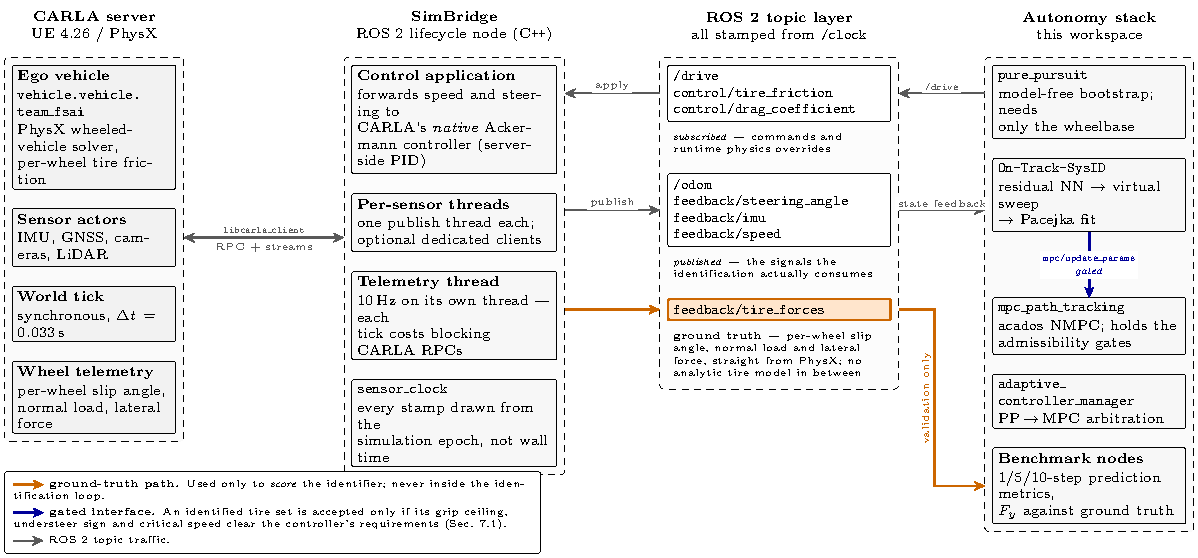
\includegraphics[width=\textheight]{Figures/bridge_architecture.pdf}
\caption{Architecture of the \bridge{} ROS~2 interface. The bridge links
against CARLA's C\texttt{++} client, drives the ego vehicle through CARLA's
native Ackermann controller, and republishes state, sensors and per-wheel
telemetry on ROS~2 topics stamped from the simulation clock. The
\texttt{feedback/\allowbreak tire\_forces} path (highlighted) carries the
simulator's own per-wheel slip angle, normal load and lateral force, and is the
ground truth against which the identifier is scored.}
\label{fig:bridge}
\end{sidewaysfigure}

\begin{table}[htbp]
\caption{ROS~2 interface used by the identification and validation pipeline.
Namespace is \texttt{/sim} unless marked absolute.}
\label{tab:topics}
\centering
\scriptsize
\setlength{\tabcolsep}{3pt}
\begin{tabular}{@{}p{2.9cm}p{4.1cm}p{5.6cm}@{}}
\toprule
Topic & Type & Role\\
\midrule
\texttt{/odom} & \texttt{nav\_msgs/Odometry} & State $v_{x},v_{y},\omega$; twist is body-frame\\
\texttt{feedback/\allowbreak steering\_angle} & \texttt{std\_msgs/Float32} (deg) & Achieved road-wheel angle $\delta$\\
\texttt{feedback/imu} & \texttt{sensor\_msgs/Imu} & $a_{x},a_{y}$ for the friction warm-start\\
\texttt{feedback/\allowbreak tire\_forces} & \texttt{sim\_manager\_\allowbreak msgs/\allowbreak TireForces} & Per-wheel $\alpha$, $F_{z}$, $F_{y}$, $\mu$, $\omega_{w}$, $\kappa$: \textbf{ground truth}\\
\texttt{feedback/\allowbreak vehicle\_physics} & \texttt{std\_msgs/String} (JSON) & Live wheel parameters of Eq.~\eqref{eq:physx}\\
\texttt{feedback/speed} & \texttt{std\_msgs/Float32} & Forward speed echo\\
\texttt{feedback/motors} & \texttt{std\_msgs/String} (JSON) & Per-wheel speed/torque/brake\\
\texttt{/drive} & \texttt{ackermann\_msgs/\allowbreak Ackermann\allowbreak Drive\allowbreak Stamped} & Control command in\\
\texttt{control/\allowbreak tire\_friction} & \texttt{std\_msgs/Float32} & Runtime grip override\\
\texttt{/clock} \emph{(abs.)} & \texttt{rosgraph\_msgs/\allowbreak Clock} & Simulation time base\\
\bottomrule
\end{tabular}
\end{table}

\paragraph{Per-wheel ground truth}
\texttt{feedback/\allowbreak tire\_forces} carries CARLA's own
\texttt{Wheel\-TelemetryData} in wheel order [FL, FR, RL, RR]. No analytic tire
model exists inside the bridge, so nothing on this topic can disagree with the
physics the vehicle is driven by. Four measured properties bound what may be
read off it. (i)~Only \texttt{lateral\_force} is force ground truth; it is the
channel every validation in this paper uses.
(ii)~\texttt{longitudinal\_force} is a friction-capacity report rather than a
measurement, tracking $\mu F_{z}$ and correlating with $ma_{x}$ at \num{0.04},
and \texttt{wheel\_torque} is an exact identity of it. (iii)~Below
\SI{0.5}{\meter\per\second} the publisher zeroes slip angle and both forces
while the normal load stays live, so the identifier gates on the all-zero
pattern as well. (iv)~The slip angle needs no sign change across the boundary;
that was verified, not assumed.

Figure~\ref{fig:frames} states the conventions the rest of the paper assumes.
CARLA inherits Unreal's left-handed world while every ROS~2 topic follows
REP-103~\cite{rep103} and the identification equations are written in the body
frame with $\alpha$ and $F_{y}$ positive to the left, the SAE-style axis
convention~\cite{saej670,pacejka2012book}. The bridge is a per-channel
conversion rather than a single transform, and the trap is that the tire
telemetry's slip angle needs \emph{no} sign change, because the frame flip and
CARLA's own convention cancel: an error there is invisible in the states and
inverts the identified curve, so it was checked against a slip angle rebuilt
from the chassis state in a steady \SI{4}{\meter\per\second} turn, equal in
magnitude to within \SI{2}{\percent} front and \SI{15}{\percent} rear.

\begin{figure}[htbp]
\centering
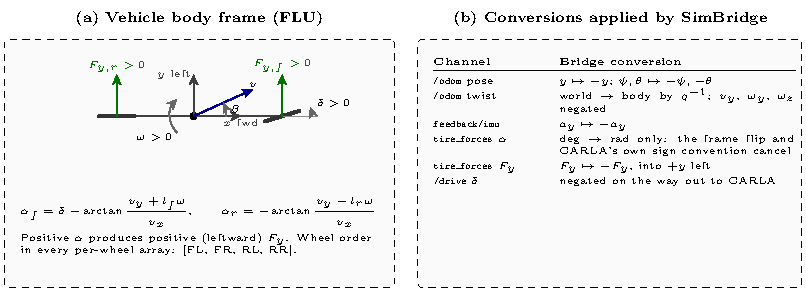
\includegraphics[width=\textwidth]{Figures/frames.pdf}
\caption{Frame and sign conventions across the simulator--ROS~2 boundary.
(a) All identification quantities are defined in the body frame:
$x$ forward, $y$ left, $\omega$ and $\delta$ positive counter-clockwise, and
slip angle and lateral force positive to the left, so that a positive $\alpha$
produces a positive $F_{y}$~\cite{saej670}. (b) The conversion applied per
channel. The slip angle of the tire telemetry is the one exception that needs
no sign change, because the frame flip and CARLA's own convention cancel.}
\label{fig:frames}
\end{figure}

\section{Reference Implementation}
\label{sec:refimpl}

The identification package, the ROS~2 bridge and the controller stack used in
this paper are released as open source. \sysid{} extends the published
baseline~\cite{ontrack2025} (upstream:
\url{https://github.com/ForzaETH/On-Track-SysID}) and is distributed under the
MIT licence that upstream's package manifest declares. \bridge{} is a separate
GPL-3.0 package, and the MPC and benchmarking packages ship with it, together
with the scenario definitions, the exported result CSV files, and the figure
and sweep generators. The links to \bridge{} and to the project repository
identify the authors and are therefore withheld from this blinded manuscript;
they are on the title page and will be printed here in the accepted version.

\end{appendices}

\backmatter

\bmhead{Supplementary information}

This article has accompanying supplementary information, submitted as a
separate document (\texttt{supplementary.pdf}). It holds the residual model's
physics-augmented inputs and objective, the temporal residual and the exact
reduction of its cost, the per-phase identification timing, the axis-by-axis
comparison against the baseline pipeline as published, and the supporting
result figures. No argument in this article depends on it.

\section*{Declarations}

\begin{itemize}
\item \textbf{Data Availability}
Every figure and table in Section~\ref{sec:results} is exported together with
the CSV file holding its samples, and the cross-run comparison reads those CSV
files rather than re-deriving any metric. The scenario definitions, the
exported result CSV files, and the figure and sweep generators are released
with the source repositories named in Appendix~\ref{sec:refimpl}. The
repository links are withheld from this blinded manuscript and are on the
title page.

\item \textbf{Code Availability}
The identification package, the simulator bridge, and the model predictive
control and benchmarking packages are released as open source; see
Appendix~\ref{sec:refimpl}. The identification package extends the released
baseline of~\cite{ontrack2025} under the MIT licence that its package manifest
declares; the simulator bridge is GPL-3.0. The two run as separate ROS~2
overlays communicating only over ROS~2 topics and services, and neither links
against the other.

\item \textbf{Conflict of Interest}
The authors declare no competing interests relevant to the content of this
article.

\item \textbf{Ethics approval}
Not applicable. All results in this article are obtained in simulation. No
experiment involved human subjects, personal data, live vertebrates, or the
operation of a physical vehicle.

\item \textbf{Funding}
Not applicable. This work received no specific grant from any funding agency in
the public, commercial, or not-for-profit sectors.

\item \textbf{Author Contributions}
Stated on the separate title page, as the journal's double-blind procedure
requires.
\end{itemize}

\end{document}
